%-------------------- begin preamble ----------------------

\documentclass[a4paper,twocolumn]{article}

\usepackage{relsize,makeidx,color,setspace,amsmath,amsfonts,amssymb, mathtools}
\usepackage[table]{xcolor}
\usepackage{bm,ltablex,microtype}
\usepackage{hyperref}
\usepackage{fontawesome}   
\usepackage[pdftex]{graphicx}
\usepackage{tcolorbox}
\usepackage[font=small, labelfont=bf, font=footnotesize]{caption}
\usepackage{subcaption}
\usepackage{float}
\usepackage[title]{appendix}
\usepackage{stfloats}
\usepackage{enumitem}
\usepackage{setspace}

\DeclarePairedDelimiter\set\{\}
\newcommand\numberthis{\addtocounter{equation}{1}\tag{\theequation}}

\newcolumntype{P}[1]{>{\centering\arraybackslash}p{#1}}
\newcommand{\R}{\mathbb{R}}
\newcommand{\E}{\mathbb{E}}
\newcommand{\y}{\mathbf{y}}
\newcommand{\ytilde}{\mathbf{\widetilde{y}}}
\newcommand{\X}{\mathbf{X}}
\newcommand{\B}{\boldsymbol{\beta}}
\newcommand{\Bhat}{\boldsymbol{\hat{\beta}}}
\newcommand{\eps}{\boldsymbol{\varepsilon}}
\newcommand{\norm}[1]{\left\lVert#1\right\rVert}
\begin{titlepage}
    \begin{center}
        \Huge
        \textbf{Classification of heart disease presence using Decision Trees, Random Forests, Gradient Boosting and Adaptive Boosting}\\
        \vspace{0.5cm}
        \LARGE
        FYS-STK3155 - Project 3\\
        Didrik Spanne Reilstad
        
        \vspace{0.5cm}
        \begin{abstract}
            \noindent Comparison of Decision Trees, Random Forests, Gradient Boosting and Adaptive Boosting as classification models for prediction heart disease presence
        \end{abstract}
        \vspace{0.8cm}
        
\includegraphics[scale=0.16]{heart.jpg}
    \end{center}
\end{titlepage}

\begin{document}
\raggedbottom
\begin{center}
    \small \textbf{Github}
    
    \vspace{0.2cm}
    
    \faGithub \ \small \href{https://github.com/dreilstad/FYS-STK3155/tree/master/Project3}{github.com/dreilstad/FYS-STK3155/Project3}
\end{center}
\vspace{0.5cm}
\section{Introduction}
According to the World Health Orgainization\cite{who}, cardiovascular diseases (CVDs) are the number one leading cause of death globally. CVDs include disorders of the heart and blood vessels. It is estimated that 17.9 million die from cardiovascular diseases each year. 4 out of 5 CVD deaths are due to heart attacks and strokes. A third of these deaths, are premature deaths of people under the age of 70. In order to prevent premature deaths of people with cardiovascular diseases, early detection, counselling and medicines are needed.\\
\\
Early detection of heart disease in people is an incredibly important tool. To facilitate early detection in as many people as possible we need to automate the classification of heart disease presence. Since heart disease is a matter of life and death, the machine learning methods used needs to predict heart disease presence with a high degree of accuracy. These methods can also help doctors and practitioners better understand the symptoms related to heart disease. For example, the authors of a recent article\cite{introarticle} on classification models for heart disease prediction was able to achieve an accuracy of $98.7\%$ using Random Forests.\\
\\
The focus of this project is similar to the aforementioned article. To study and compare the performance of classification models in predicting heart disease presence. The machine learning models studied are Decision Trees, Random Forests, Gradient Boosting and Adaptive Boosting. We use the library from Scikit-Learn\cite{scikit} to apply these models to the dataset. Additionally we look at Principal Component Analysis (PCA) and the correlation matrix to attain a better understanding of our datatset. All code used to produce the results presented in this report, can be found in the linked GitHub repository.\\
\\
The following sections of the report starts with presenting the theory behind the different classification models and also Principal Component Analysis. Subsequently the heart disease dataset used is explained in more detail. Next the results are presented and discussed. The report rounds off with the main findings of the project and future directions.
\section{Method}
This section outlines the theory behind the classification models Decision Trees, Random Forests, Gradient Boosting and Adaptive Boosting. Also the theory behind Principal Component Analysis is presented along with the metrics used to evaluate and compare each classification model.
\subsection{Principal Component Analysis}
Principal Component Analysis (PCA) is a method used to reduce the dimensionality of large datasets by reducing the number of independent variables/features. The dimensionality reduction comes at the expense of lower accuracy, but in return the analysis of the data becomes easier and faster when redundant or less important variables are left out. The problem is balancing the number of features and the possible loss of information in the data when reducing the dimensionality. The goal of PCA is essentially to reduce the number of features while also retaining and preserving as much information in the data as possible.\\
\\
The first step of the Principal Component Analysis algorithm is to standardize the values for each feature. The dataset is organized in a design matrix $\X$ of size $n \times p$ where the columns of $\X$ represent the features $x_{i}$ and the rows are the samples. The standardization of the values for feature $i$ is done by
\begin{align}
    \mathbf{x}_{i} := \frac{\mathbf{x_{i} - \mu}}{\sigma}
\end{align}
where $\mu$ is the mean and $\sigma$ is the standard deviation. The reason why this is an important step, is because PCA is sensitive to the variances of the features and the features with a larger range of values would dominate the features with a smaller range of values. Therefore the values are standardized such that each feature contributes equally when performing the PCA.\\
\\
Next, the covariance matrix is calculated. The covariance matrix is used to understand if there is any relationship between the features, or more specifically how the features vary from the mean w.r.t. each other. This can be used to find features that are highly correlated and therefore contain redundant information. The covariance matrix, or correlation matrix when scaled, is a symmetric matrix of size $p \times p$ where p is the number of features. The general covariance matrix $\mathbf{C}$ is defined as
\begin{align}
    \mathbf{C} &= \frac{1}{n - 1}\X^{T}\X\\
    \mathbf{C} &= \setlength\arraycolsep{2pt}\begin{bmatrix} 
    var[{\mathbf{x}_{0}}] & cov[\mathbf{x}_{0}, \mathbf{x}_{1}] & \dots & cov[\mathbf{x}_{0}, \mathbf{x}_{p-1}]\\
    cov[\mathbf{x}_{1}, \mathbf{x}_{0}] & var[\mathbf{x}_{1}] & \dots & cov[\mathbf{x}_{1}, \mathbf{x}_{p-1}]\\
    \vdots & \vdots & \ddots & \vdots\\
    cov[\mathbf{x}_{p-1}, \mathbf{x}_{0}] & cov[\mathbf{x}_{p-1}, \mathbf{x}_{1}] & \dots & var[{\mathbf{x}_{p-1}}]
    \end{bmatrix}
\end{align}
The covariance matrix $C$ tells us that if the sign of $cov[\mathbf{x}_{i}, \mathbf{x}_{j}]$ is positive, then the features $i$ and $j$ are correlated, and inversely correlated if the sign is negative.\\
\\
Next step is to compute the eigenvectors and eigenvalues of the covariance matrix $C$ in order to find the principal components. The principal components are "new features" constructed as a linear combination of the initial features. The idea is to construct these principal components such that they are uncorrelated and we therefore remove redundant information and retain most of the essential information into the first principal component. The the second principal component is constructed trying to maximize the remaining information, and so on until we reach the $k$ principal component. Meaning we construct $k$ principal components, where $k \leq p$. We end up with a new $k$-dimensional feature subspace of the original $p$-dimensional feature space.\\
\\
Geometrically, the principal components is the line, or hyperplane when more than two features, where the \textit{reconstruction error} is minimized\cite{hastie} or in other words the most information is retained. In this project we use PCA to better understand which features are the most important when predicting heart disease presence by studying the explained variance ratios. The explained variance ratios is calculated using the eigenvalues and shows us how much information about the data can be attributed to each principal component.\\
\\
Seeing as $n\gg p$, where in our case $n = 297$ and $p = 13$, PCA is rarely used to reduce the dimensionality of the dataset. Applying PCA to reduce the dimensionality is normally only used when $p \gg n$. Therefore we keep the 13 features in order to achieve the highest accuracy possible.
\begin{figure}[ht]
    \centering
    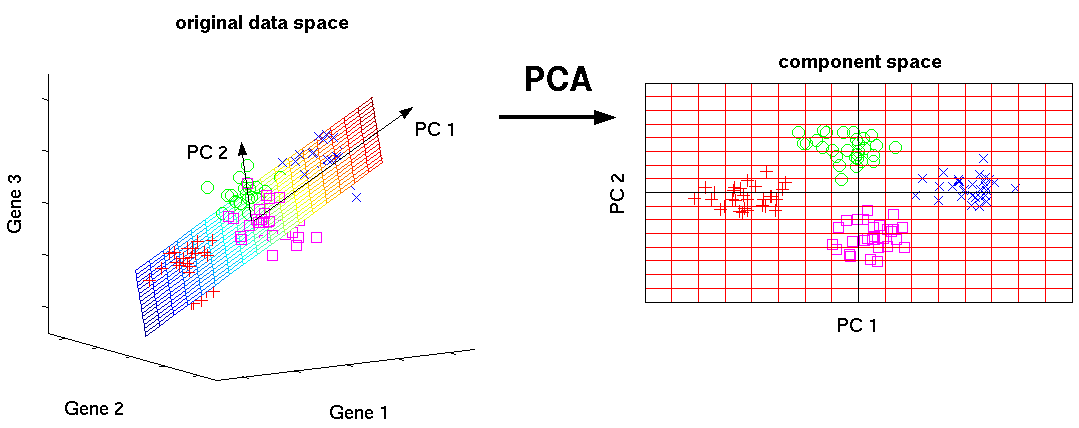
\includegraphics[width=\columnwidth]{fig_pca_principal_component_analysis.png}
    \caption{Visualization using PCA to reduce three initial features to two "new features", i.e. principal components. \href{http://www.nlpca.org/pca_principal_component_analysis.html}{http://www.nlpca.org/pca\_principal\_component\_analysis.html}}
    \label{fig:1}
\end{figure}
\subsection{Decision Trees}
A decision tree is a basic and simple algorithm that is used for both regression and classification problems, and also is used to build more complex models such as Random Forests or Gradient Boosting.
\begin{figure}[ht]
    \centering
    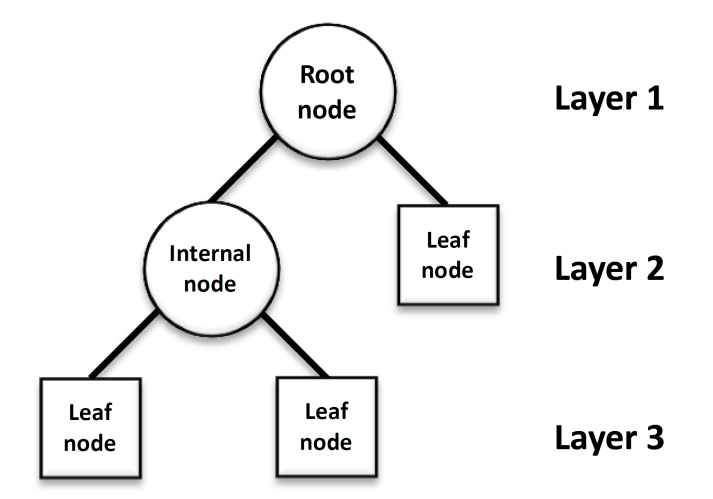
\includegraphics[width=\columnwidth]{decision_tree.png}
    \caption{Visualization of the structure of a decision tree. \href{https://www.researchgate.net/figure/Basic-structure-of-a-decision-tree-All-decision-trees-are-built-through-recursion_fig3_295860754}{https://www.researchgate.net/figure/Basic-structure-of-a-decision-tree}}
    \label{fig:2}
\end{figure}\\
Figure \ref{fig:2} shows the structure of a decision tree. A decision tree consists of a single root node, internal nodes and leaf nodes. The root nodes and internal nodes represent conditionals or tests using the features. For example, go to the right subtree if age $> 70$, and left if not. The leaf nodes represent the prediction of the decision tree after going through the conditionals in the internal nodes with the values of an instance/sample. The leaf nodes will have different predictions depending on the path from the root node through the internal nodes to the leaf node.\\
\\
The process of structuring and training a decision tree using a top-down approach with the ID3 algorithm is as follows:
\begin{enumerate}
    \item Start with a dataset containing $n$ instances/samples with $p$ features and the corresponding true target values.
    \item Create $p$ trees with only a root node and two leaf nodes, where each feature is used in the root node. Evaluate the performance using the training samples. This evaluation score is called the impurity because none of the trees will correctly classify all the samples. The feature with the tree achieving the lowest impurity will become the feature used in the root node. This feature best separates the two possible classes/outcomes.
    \item Next step is to continuously split along the features on the left side of the root node and at each split evaluate the impurity. The feature with the lowest impurity becomes the features used int he internal node. This continues down the branch until all features has been assigned to an internal node. We repeat the process for the rights side of the root node.
    \item Now the decision tree has been constructed with the features placed at the optimal nodes. We can feed samples through the tree to the leaf nodes to get a prediction.
\end{enumerate}
The impurity is measured by either using the Gini index or the Entropy. These metrics are defined as
\begin{align}
    Gini &= \sum_{k = 1}^{K} p_{k}(1 - p_{k})\\
    Entropy &= \sum_{k = 1}^{K} p_{k} log(p_{k})
\end{align}
where $p_{k}$ is the probability of class $k$, and $K$ is the total number of classes. The performance of the decision tree is unlikely to change depending on which metric is chosen, but the gini index is often more used due to not having to calculate the $log$ which takes longer computationally.\\
\\
Some of the advantages of using a decison tree is that it is a simple decision-making model which humans can relate to and understand. Also decision trees do not require the dataset to be normalized/scaled. Can handle both numeric data and categorical data for regression and classification problems.\\
\\
Still, decision trees are usually outperformed by some of the other machine learning models. Can also be prone to overfitting to the training data and is also sensitive to changes in the dataset. In an attempt to prevent overfitting, methods like bagging and boosting is used to improve the performance. These methods are the basis for the other classification models presented in the subsequent sections.
\subsection{Random Forests}
Random forests are classified as an ensemble learning method for regression and classification problems. Ensemble learning methods combine multiple machine learning algorithms in order to achieve an even higher performance. Random forests improves on decision trees by constructing multiple trees outputs the mode of the classes for classification or the mean prediction for regression of the individual trees. The mode of the classes is the value/class that predicted most often by the collection of trees. Random forests does not overfit to the training data as much as decision trees, and generally outperforms decision trees.\\
\\
A random forest is a variant of a bagged decision tree. Bagging, or boostrap aggregating, is a general model averaging approach. In the context of decision trees on a classification problem, bagging works by using bootstrap to generate $B$ different training set from the original training set. $B$ decision trees are constructed and trained on the corresponding generated training set. The mode of the classes is the output from a bagged decision trees.\\
\\
Random forests improves on bagged decision trees by reducing the number of features used when splitting in the construction of a decision tree. Whereas a bagged decision tree uses all $p$ features, a random forest tree only uses a random sample of $m$ features to split on from the full set of $p$ features. For classification, the size of $m$ is usually chosen to be $m \approx \sqrt{p}$.\\
\\
This means the random forest trees constructed are not "fully grown" and does not contain all $p$ features. The reason why generally will outperform bagged decision trees is because when the dataset contains one feature that is "stronger" than the rest, all of the bagged tree will use this feature as the root node. This will result in all the bagged trees looking similar and the output from each bagged tree will be highly correlated. When averaging over highly correlated output, the high variance as a result of overfitting is not reduced.\\
\\
By limiting the splits to only a subset of the features, the random forest algorithm forces the trees to be more decorrelated. Therefore the average of the output from the random forest trees, will be less variable and more reliable. The model is more generalized and not overfitted to the training set. Random forests mainly only reduces the variance in the error.
\subsection{Boosting methods}
Boosting is an ensemble learning method which creates a strong classifier using a number of weak classifiers. The idea is to combine the output from many weak classifiers in order to achieve a strong classifier. A weak classifier is a classifier that performs only slightly better than random guessing\cite{hastie}. When using decison trees, a weak classifier is a decison tree containing only a root node and two leaf nodes. Also called a "stump". The general iterative procedure used for boosting methods is defined as
\begin{align}
    f_{m}(x) = f_{m-1}(x) + \alpha_{m}b_{m}(x)
\end{align}
where $b_{m}$ is the weak learner and $\alpha_{m}$ is the corresponding weight.
\subsubsection{AdaBoost}
Adaptive boosting, often shortened to AdaBoost, was first proposed in 1997 by Yoav Freund and Robert E. Schapire\cite{adaboost}. The method was first implemented for a binary classification problem, but has since been adapted to multiclass classification problems and regression problems. In this project we only look at the binary case. The AdaBoost algorithm works as following:
\begin{enumerate}
    \item Start by initializing all weights to be $w_{i} = 1/n$, for $i = 0,1,2,...,n-1$.
    \item Iterate from $m=1$ to M, where M is the final number of classifications:
    \begin{enumerate}[label=(\alph*)]
        \item Fit a weak classifier $G_{m}(\mathbf{x})$ to the training data using the weights $w_{i}$.
        \item Calculate the misclassification error
        \begin{align}
            \overline{err}_{m} =\frac{\sum_{i=0}^{n-1}w_{i}I(y_{i} \neq G_{m}(x_{i}))}{\sum_{i=0}^{n-1}w_{i}}
        \end{align}
        \item Calculate $\alpha_{m} = log\left(\frac{1- \overline{err}_{m}}{\overline{err}_{m}}\right)$ 
        \item Update the weights to
        \begin{align}
            w_{i} := w_{i}\cdot exp(\alpha_{m}I(y_{i} \neq G_{m}(x_{i})))
        \end{align}
    \end{enumerate}
    \item The output is 
    \begin{align}
        G(x)=sign\sum_{m=1}^{M}\alpha_{m}G_{m}(x)
    \end{align}
\end{enumerate}
$G$ is the final strong classifier where we get our output after training/fitting on the training set and $G_{m}$ is $m$'th weak classifier. The derivation of $\alpha_{m}$ is shown in Appendix \ref{app:A}.\\
\\
The AdaBoost algorithm essentially constructs weak classifiers and sequentially iterates them. For each iteration the classifiers are re-weighted to improve on the previous iteration. The weighting focuses on improving on the features or regions where the previous tree underperformed and lead to a higher misclassificaton error. The final classifer $G$ is in essence the weighted average over all the weak classifiers.
\subsubsection{Gradient Boosting}
Gradient Boosting is very similar to AdaBoost. Both algorithms trains many trees in a sequential manner and improves upon the previous tree. The Gradient Boosting algorithm works as following:
\begin{enumerate}
    \item Initialize model with a constant value
    \begin{align}
        F_{0} = \underset{\gamma}{argmin}\sum_{i=0}^{n-1}L(y_{i},\gamma)
    \end{align}
    \item Iterate from $m=1$ to $M$:
    \begin{enumerate}[label=(\alph*)]
        \item Compute the pseudo residuals $r_{im}$, for $i = 1, ..., n$
        \begin{align}
            r_{im} = - \left[\frac{\partial L(y_{i}, F(x_{i}))}{\partial F(x_{i})}\right]_{F(x)=F_{m-1}(x)}
        \end{align}
        \item Fit a weak learners $f_{m}(x)$ to the pseudo residuals by training it on the training set $\{(x_{i}, r_{im})\}_{i=0}^{n-1}$, with the pseudo residuals as targets.
        \item Compute the multiplier $\gamma_{m}$
        \begin{align}
            \tiny
            \gamma_{m}=\text{\footnotesize$ \underset{\gamma}{argmin}\sum_{i=0}^{n-1}L(y_{i},F_{m-1}(x_{i})+\gamma f_{m}(x_{i}))$}
        \end{align}
        \item Update the model $F_{m}$
        \begin{align}
            F_{m}(x)=F_{m-1}(x) + \eta\gamma_{m}f_{m}(x)
        \end{align}
        where $\eta$ functions as a shrinkage parameter, that prevents overfitting to the training set.
    \end{enumerate}
    \item The output is $F_{M}(x)$
\end{enumerate}
The pseudo residuals are the difference between the observed values and the predicted values. When using Gradient Boosting for binary classification we use the negative log-likelihood as loss function. The negative log-likelihood is defined as
\begin{align}
    L = -\sum_{i=0}^{n-1}y_{i}\cdot log(p_{i})+(1-y_{i})\cdot log(1-p_{i})
\end{align}
where $y_{i}$ is the true observed value and $p_{i}$ is the predicted probability.\\
\\
The difference between Gradient Boosting and AdaBoost is that Gradient Boosting is not limited to only "stumps" as weak learners and can have larger decision trees. AdaBoost focuses the training on the misclassified observations, while Gradient Boosting focuses on minimizing the loss function $L$ of the weak learners. Often AdaBoost is seen as a special case of Gradient Boosting using a specific loss function, which is the exponential loss as seen in equation (8). Gradient Boosting is more flexible and more general.\\
\\
Compared to Random Forests, which mainly reduces the variance\cite[p.~588]{hastie}, boosted methods also reduce the bias by improving the regions where the previous learner underperformed. This is the reason why when comparing the performance of Random Forests to boosting methods, boosting methods can on certain problems outperform Random Forests.
\subsection{Model selection and assessment}
To measure the performance of a classification model we look at the accuracy score. In addition we visualize the classifiers by using the confusion matrix and plot the ROC-curve. 
\subsubsection{Accuracy score}
For binary classifiaction we use the accuracy score to measure the proportion of correct classifications among the total number classifications. The accuracy is defined as
\begin{align}
    Accuracy = \frac{TP + TN}{TP + TN + FP + FN}
\end{align}
where true positive (TP) is the patients who had heart disease presence and were correctly classified, true negative (TN) is the patients who did not have heart disease presence and were correctly classified, false positive (FP) is the patients who did not have heart disease presence but were incorrectly classified and false negative (FN) is the patients who had heart disease presence but were incorrectly classified.
\subsubsection{Confusion matrix}
The confusion matrix is a helpful way to visualize the proportion of the total classifications that were correct and the proportion that were incorrect. Figure \ref{fig:3} shows an example of a confusion matrix. Often the confusion matrix is normalized to values between 0 and 1 in each cell to easier compare the ratios.
\begin{figure}[ht]
    \centering
    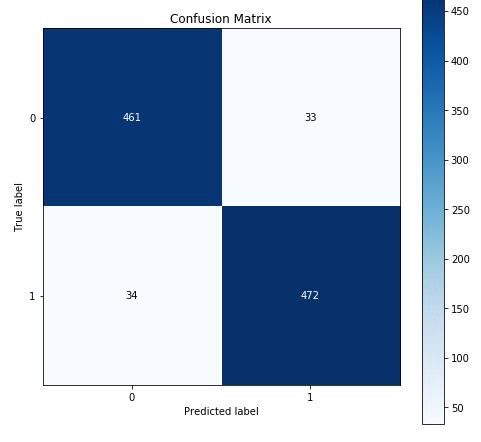
\includegraphics[width=\columnwidth]{confusion_matrix.jpeg}
    \caption{Example of non-normalized confusion matrix. Source: \href{https://towardsdatascience.com/metrics-and-python-ii-2e49597964ff}{https://towardsdatascience.com/metrics-and-python-ii-2e49597964ff}}
    \label{fig:3}
\end{figure}
\subsubsection{ROC curve}
A reciever operating characteristic curve, ROC curve, plots the true positive rate (TPR) against the false positive rate (FPR). The true positive rate is also known as the sensitivity or recall, and the false positive rate is also known as the fall-out. They are defined as
\begin{align}
    TPR &= \frac{TP}{TP + FN}\\
    FPR &= \frac{FP}{FP + TN}
\end{align}
In addition to plotting the TPR against the FPR, we calculate the area under the ROC curve to get an aggregate measure of the performance of the model. This value is often referred to as the AUC and can be interpreted as the probability that the model correctly classifies a random sample. The AUC has a value between 0 and 1, where $100\%$ correct classification means an AUC score of 1.0. Figure \ref{fig:4} shows an example of a ROC curve.
\begin{figure}[ht]
    \centering
    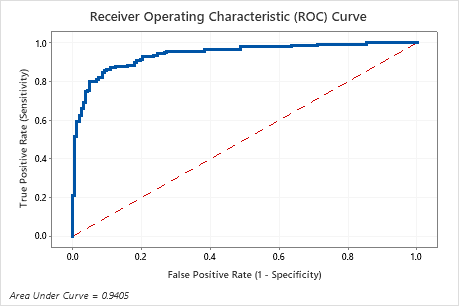
\includegraphics[width=\columnwidth]{roc_curve.png}
    \caption{Example of a ROC curve in blue and the dashed red line represents random guessing. Source: \href{https://support.minitab.com/en-us/minitab/19/help-and-how-to/statistical-modeling/regression/how-to/fit-binary-logistic-model/interpret-the-results/all-statistics-and-graphs/receiver-operating-characteristic-roc-curve/}{https://support.minitab.com/en-us/minitab/19/receiver-operating-characteristic-roc-curve/}}
    \label{fig:4}
\end{figure}
\subsubsection{Parameter search and resampling technique}
To improve the certainty of the model assessment, k-fold cross validation is used as a resampling technique. Due to not having a large amount of data to train, using resampling techniques can help mitigate this by reusing the dataset. When working with classification methods such as decision trees, random forests and boositng methods, there are a lot of parameters to tune in order to find the optimal model. \\
\\
Therefore Scikit-Learn's $\verb"GridSearchCV"$ functionality is used in order to find the optimal parameters more efficiently because the parameter search can be parallelized. The functionality uses cross validation as resampling technique. After performing a gridsearch, the best model is tested on a untouched test set. Thus, the "test" set in cross validation becomes a validation set to select the best model.
\subsubsection{k-fold Cross Validation}
K-fold cross validation is the technique of dividing the dataset into $k$ folds, or subsets, and assigning fold $i$ to be the test set and the remaining folds to be the training set. The dataset is randomly shuffled for each division of folds. We fit a model on the training folds and predict a model against the test fold. The performance score for the model is saved for later. This process is repeated $k$ times where each fold is the test fold once.\\
\\
K-fold cross validation is used as a resampling technique for model assessment. It is used to estimate the mean performance of a model with a given learning method.
\section{Dataset}
The dataset used is a heart disease dataset from the UCI Machine Learning Repository, more specifically the Cleveland dataset\cite{dataset}. The original dataset contains 76 attributes, but all published articles only use a subset of 14 attributes. For almost all machine learning experiments, the Cleveland dataset is the only one that has been used. The goal is to predict the presence of heart disease (values 1,2,3,4) or absence of heart disease (value 0). We convert the problem to a binary classification problem by converting the classes 1,2,3, and 4 in the target attribute to the same class with label 1. This means when a patient is classified as having presence of heart disease, this does not indicate anything about the severity.\\
\\
Six instances of the dataset had a missing values for one or more features. Since the number of instances with mising values was low, these were removed. After processing and cleaning the data, we end up with a total of 297 instances. 160 of the instances has no heart disease presence, and 137 has heart disease presence. There is not a large difference between the number of instances for each class, meaning we are less likely to get skewed results.\\
\\
The 14 attributes, where one attribute is the target value and the remaining 13 are the explanatory features used to classify. Table \ref{tab:1} contains the explanatory features used and a short description of them.
\begin{table}[h]
    \centering
    \caption{Features of the Heart Disease dataset.}
    \label{tab:1}
    \begin{tabular}{|p{1.2cm}|p{5.5cm}|}
    \hline
        \cellcolor{gray!25} \textbf{Feature} & \cellcolor{gray!25} \textbf{Description} \\ 
        \hline\hline
        age & Age of patient in years \\ 
        \hline
        sex & Sex of patient (1 = male, 0 = female)\\
        \hline
        cp & Chest pain type (1 = typical angina$^*$, 2 = atypical angina$^*$, 3 = non-anginal pain, 4 = asymptomatic)\\
        \hline
        trestbps & Resting blood pressure (in mm Hg on admission to the hospital)\\
        \hline
        chol & Serum cholestoral in mg/dl\\
        \hline
        fbs & Fasting blood sugar $>$ 120mg/dl (1 = yes, 0 = no)\\
        \hline
        restecg & Resting electrocardiographic results\\
        \hline
        thalach & Maximum heart rate achieved\\
        \hline
        exang & Exercise induced angina$^*$ (1 = yes, 0 = no)\\
        \hline
        oldpeak & ST depression induced by exercise relative to rest\\
        \hline
        slope & The slope of the ST segment (1 = upsloping, 2 = flat, 3 = downsloping)\\
        \hline
        ca & Number of major vessels (0-3) colored by flourosopy\\
        \hline
        thal & Exercise Thallium heart scan (3 = normal, 6 = fixed defect, 7 = reversible defect)\\
        \hline
    \end{tabular}
    \text{\footnotesize{$^*$Anginal chest pain is chest pain caused by}}
    \text{\footnotesize{reduced blood flow to the heart muscles.}}
\end{table}\\
\section{Results \& Discussion}
Before testing the different classification models presented earlier, we first study the data. In appendix \ref{app:B}, the histograms for both heart disease presence and no heart disease presence is plotted for each feature. Studying the plotted histogram, we see for the feature $\verb"age"$ that those patients with heart disease presence tends to be older. Heart disease presence is especially prevalent in the interval age 55 to age 66. The reason for the drop off for higher ages is because there are less instances with patients with a higher age. If the dataset contained a higher number of instances with older patients, we would see heart disease presence dominate for these patients also. \\
\\
Also noticeable is the histograms for the feature $\verb"sex"$. Just looking at the histograms you could conclude that heart disease is more prevalent in men than women, but there number of instances of male patients versus female aptients in the dataset si skewed towards male. There are a total of 201 male instances and 96 instances female instances.
\begin{figure}[ht]
    \centering
    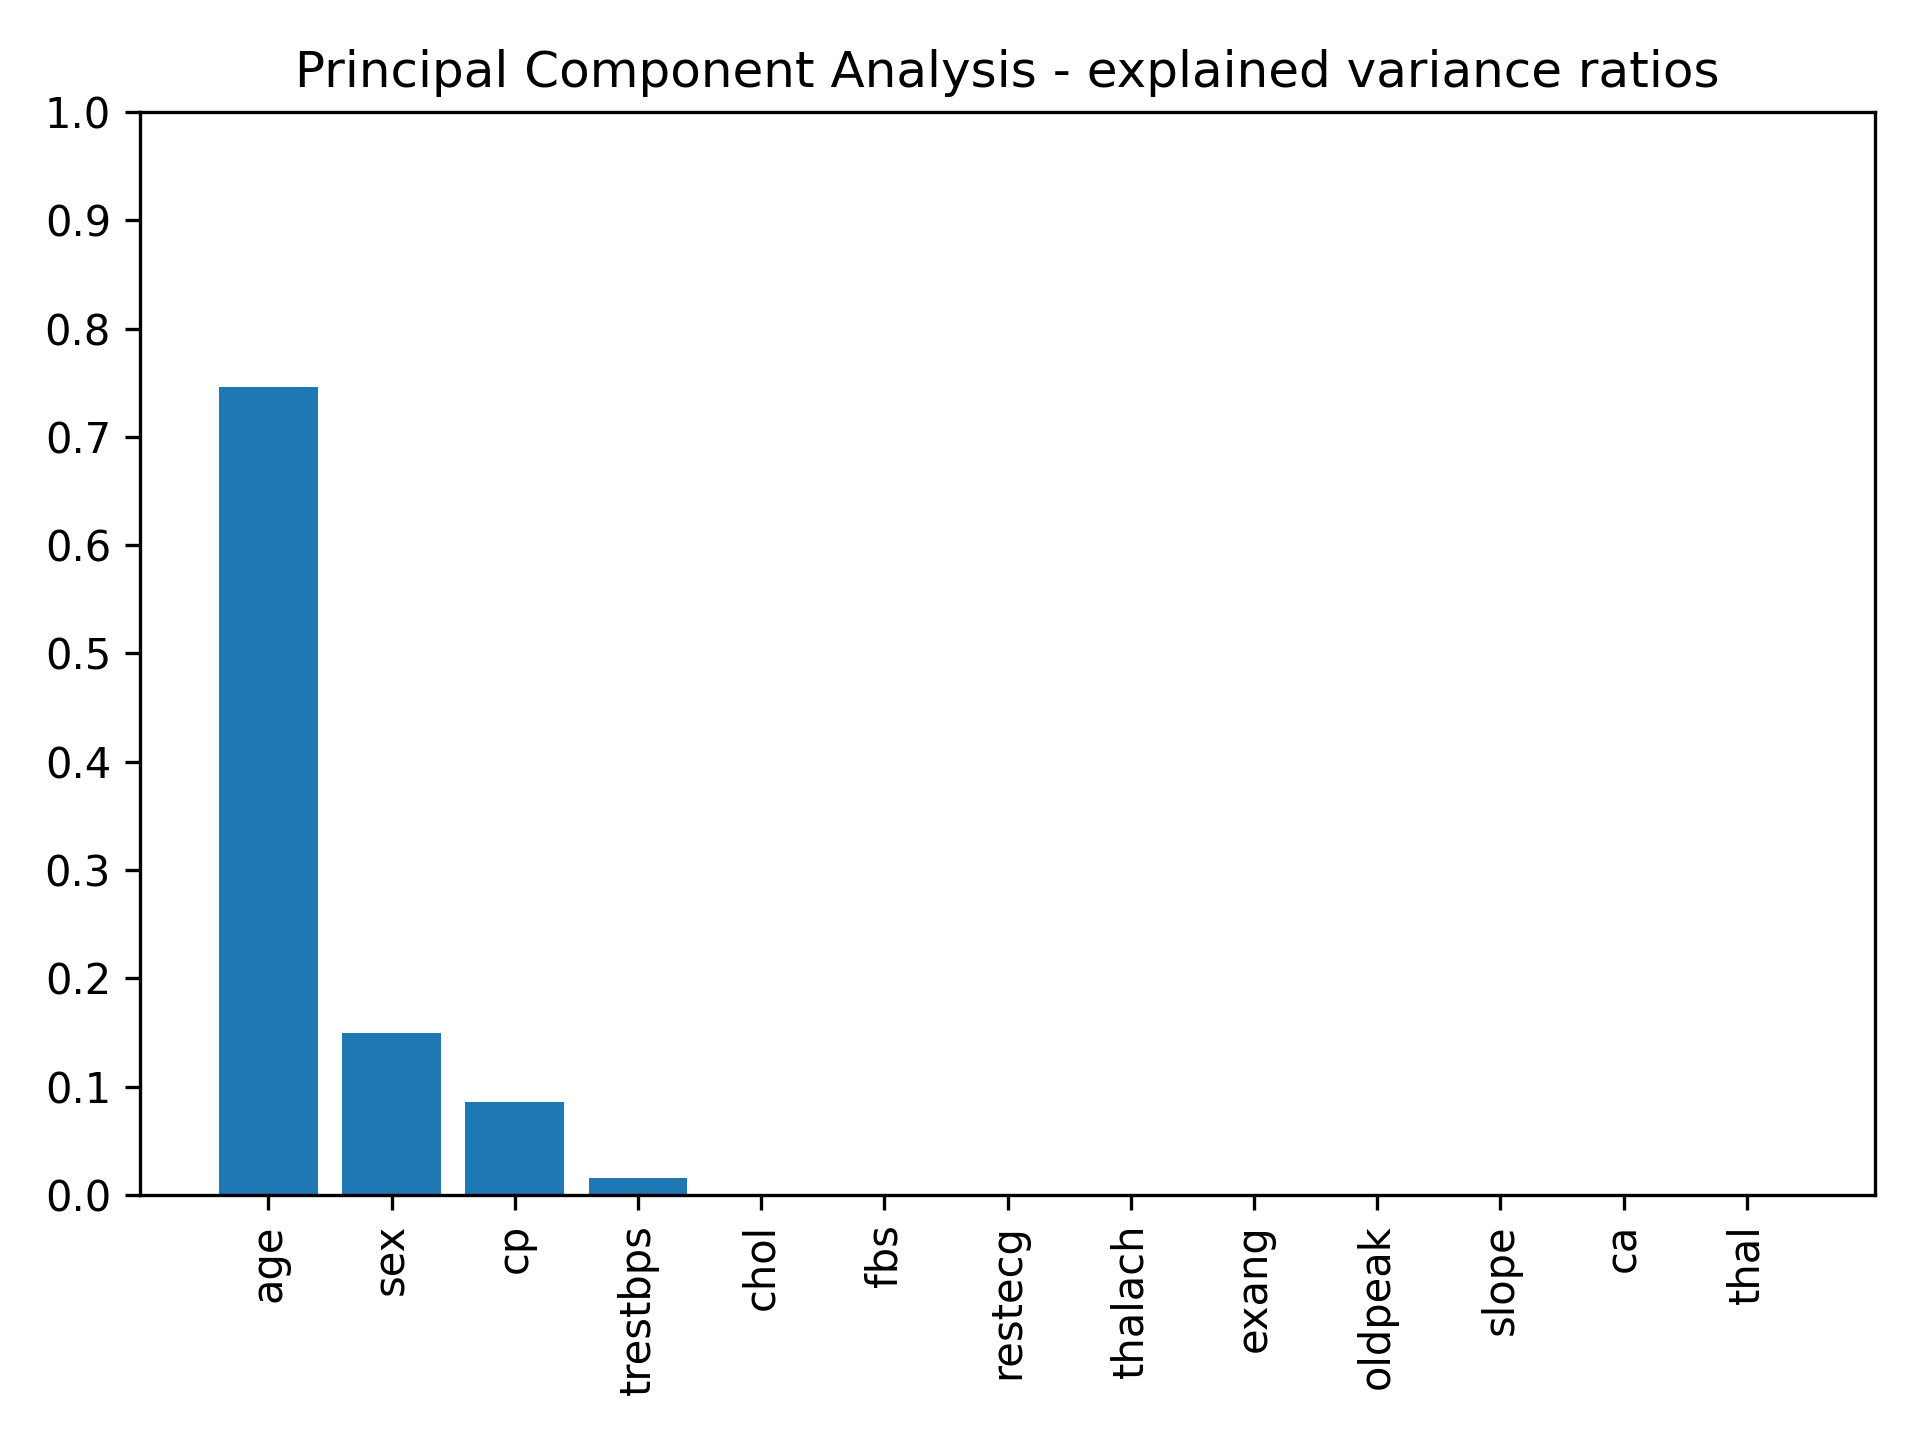
\includegraphics[width=\columnwidth]{pca_variance_ratio.png}
    \caption{Principal Component Analysis explained variance ratios for all features in the heart disease dataset.}
    \label{fig:5}
\end{figure}
\begin{figure*}[b]
    \centering
    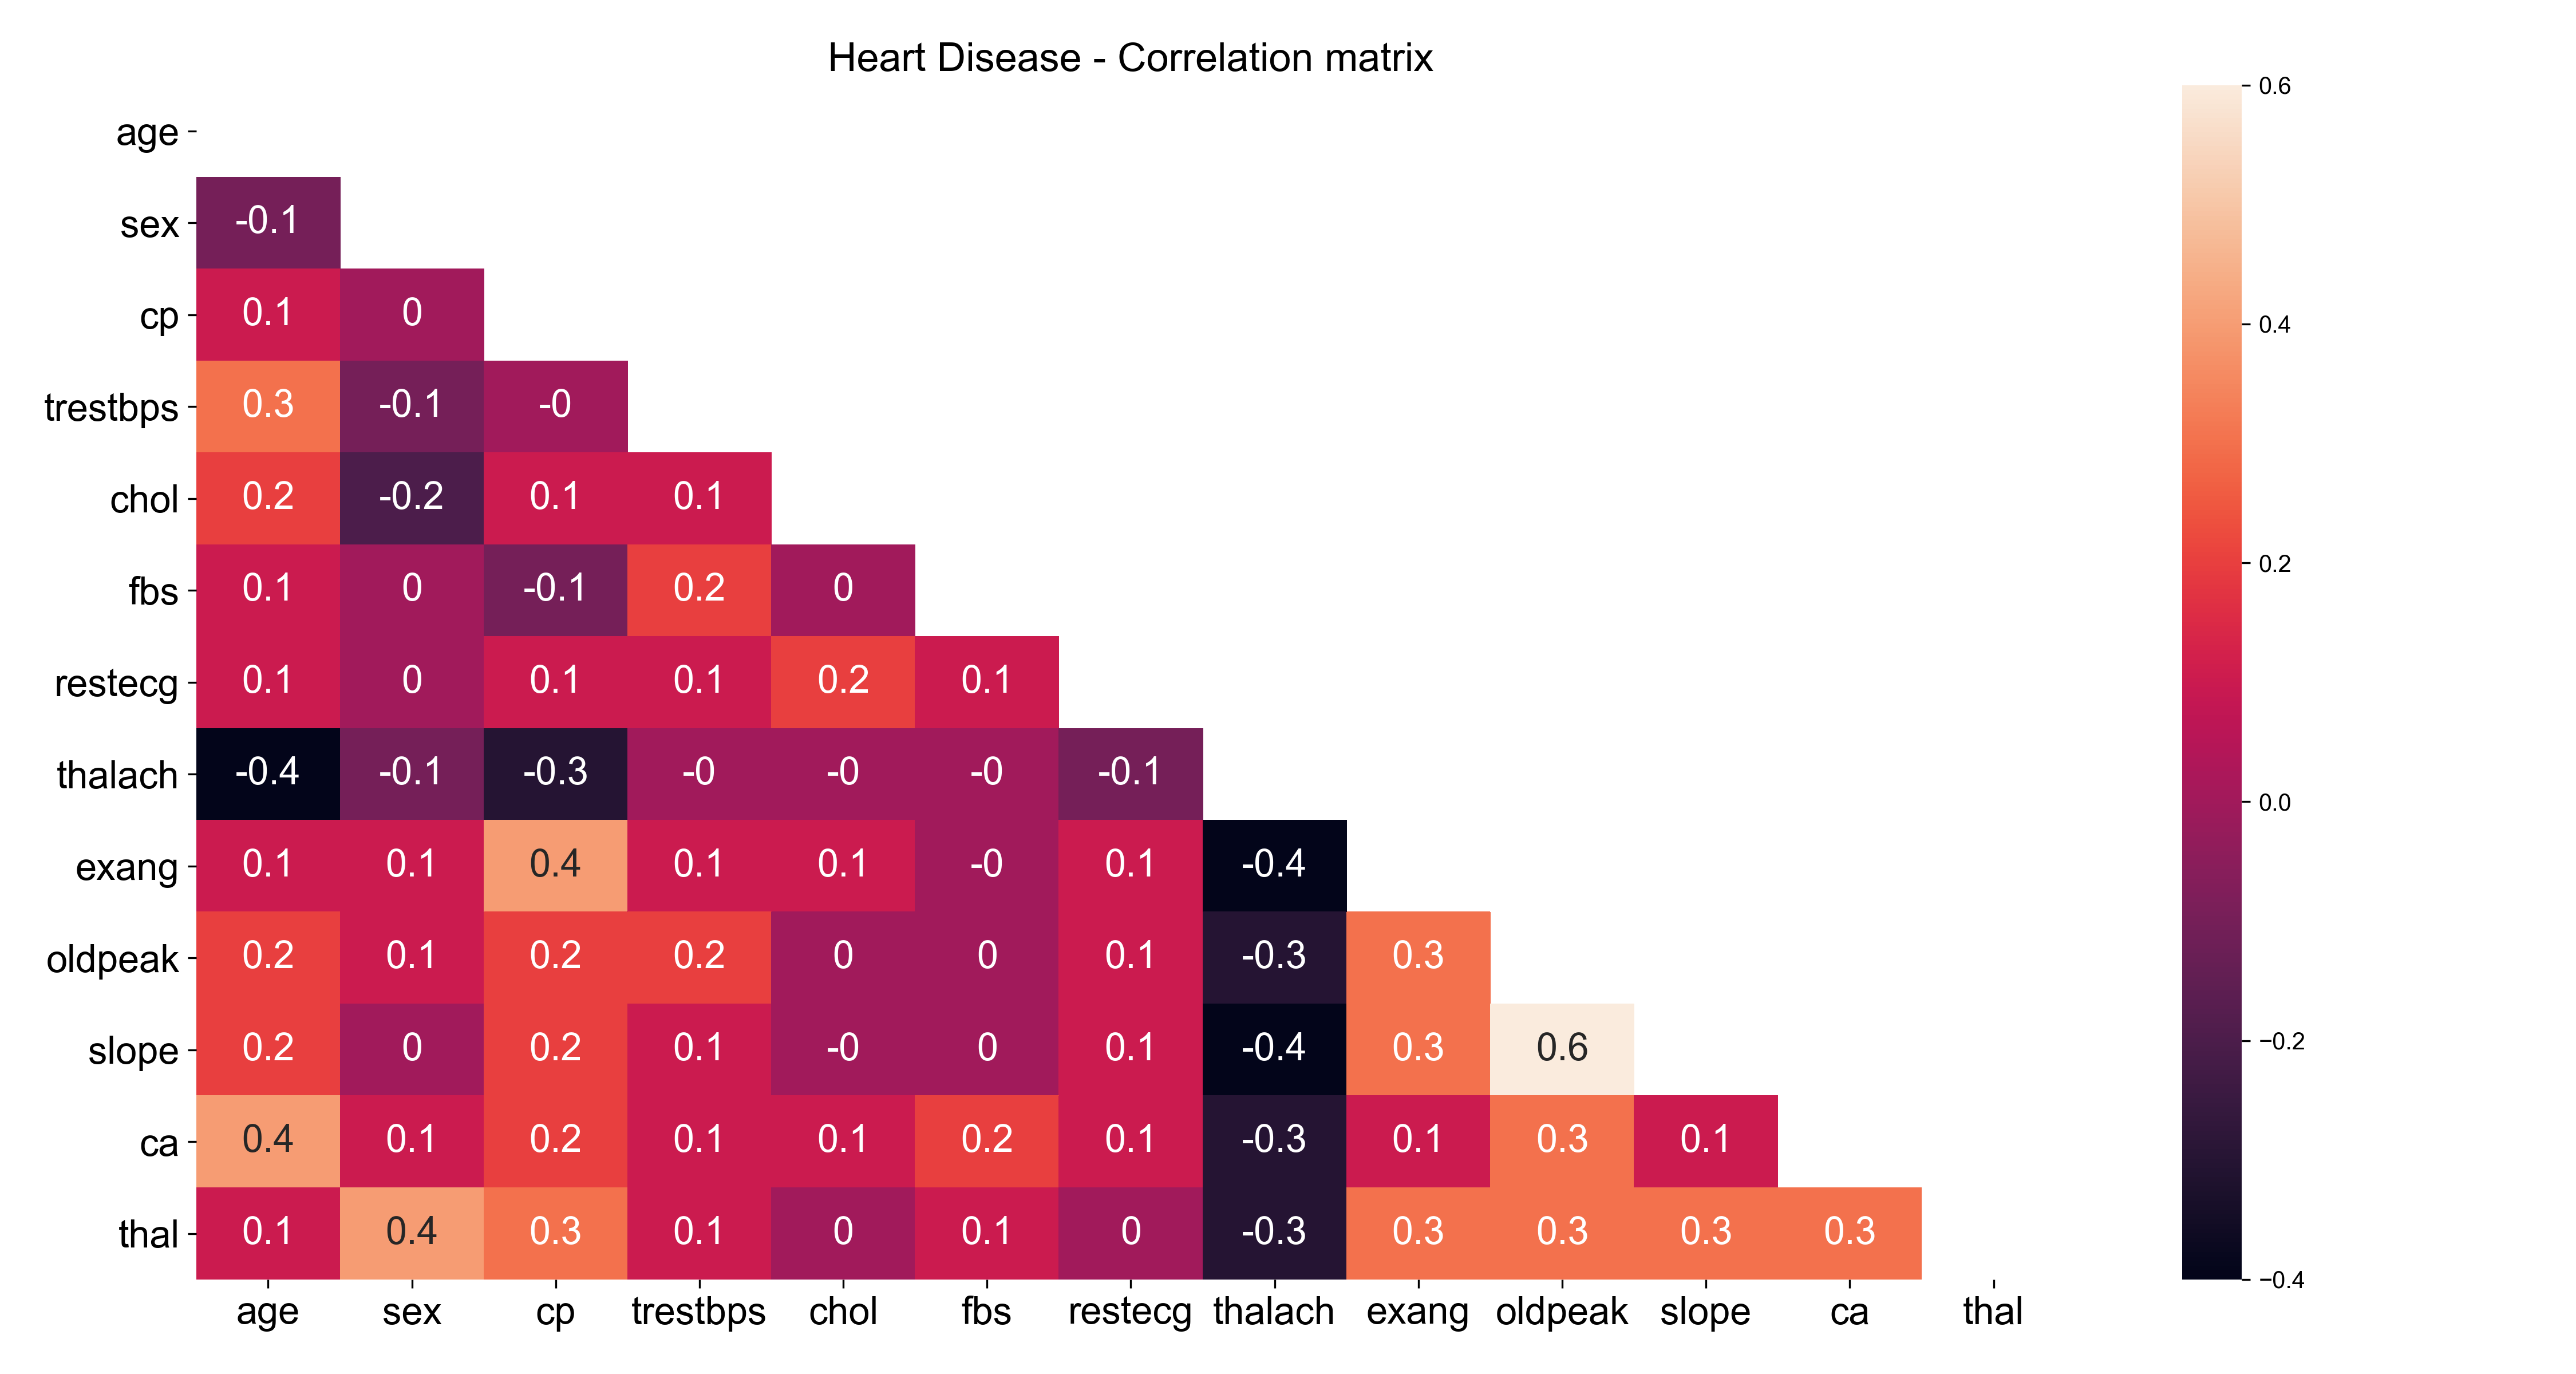
\includegraphics[width=0.95\textwidth]{heart_disease_corr_matrix.png}
    \caption{Correlation matrix for all features in the heart disease dataset.}
    \label{fig:6}
\end{figure*}\\
A superior and more informative way to see the importance of certain features compared to the others is using PCA. Figure \ref{fig:5} plots the explained variance ratio for each feature.\\
\\
As was stated earlier, the explained variance ratio is the proportion of variance that can be attributed to each feature. From figure \ref{fig:5}, we can see that $\verb"age"$ contributes approximately $0.75$. The features contributing to a lesser extent but are still important, are the features $\verb"sex"$, $\verb"cp"$ and $\verb"trestbps"$. Summing up all ratios for every feature, we get $1$. If we only sum up the first four features, we get $0.997$ which means that the remaining features could in theory be excluded while still retaining the most essential information in the dataset. Since the number of features is relatively low, there is no need to reduce the dimensionality.\\
\\
Next we examine if several of the features are correlated or not. Figure \ref{fig:6} plots the correlation matrix. The value in each cell indicates the level of correlation and the sign indicates the direction. This means a value of 0.9 indicates that two features are strongly correlated, while a value of -0.5 indicates that two features are moderately inversely correlated. \\
\\
Studying figure \ref{fig:6}, we see that none of the features are particularly correlated or inversely correlated. The highest correlation value is 0.6 for the features $\verb"oldpeak"$ and $\verb"slope"$, meaning they are moderately correlated. There are some instances of the other features being more weakly correlated or inversely correlated, such as $\verb"age"$ and $\verb"thalach"$. Most cells in the correlation matrix has a value closer to 0, meaning the features in the dataset are generally not correlated or weakly correlated.
\\
\\
Before looking at the performance of the classification models, a dataset containing uncorrelated features should theoretically only improve the performance. While it is not a given that uncorrelated features will improve the performance, it will not worsen it seeing as the more uncorrelated the features are the more information the classifier can work with. Two highly correlated features will not add any additional information, and one of them can be removed to reduce the dimensionality. \\
\\
Next we look at the performance of the different classificiation methods, starting with decision trees. Figure \ref{fig:7} plots the accuracy as a function of the $\verb"max_depth"$ parameter, which determines the maximum depth the tree can have.
\begin{figure}[ht]
    \centering
    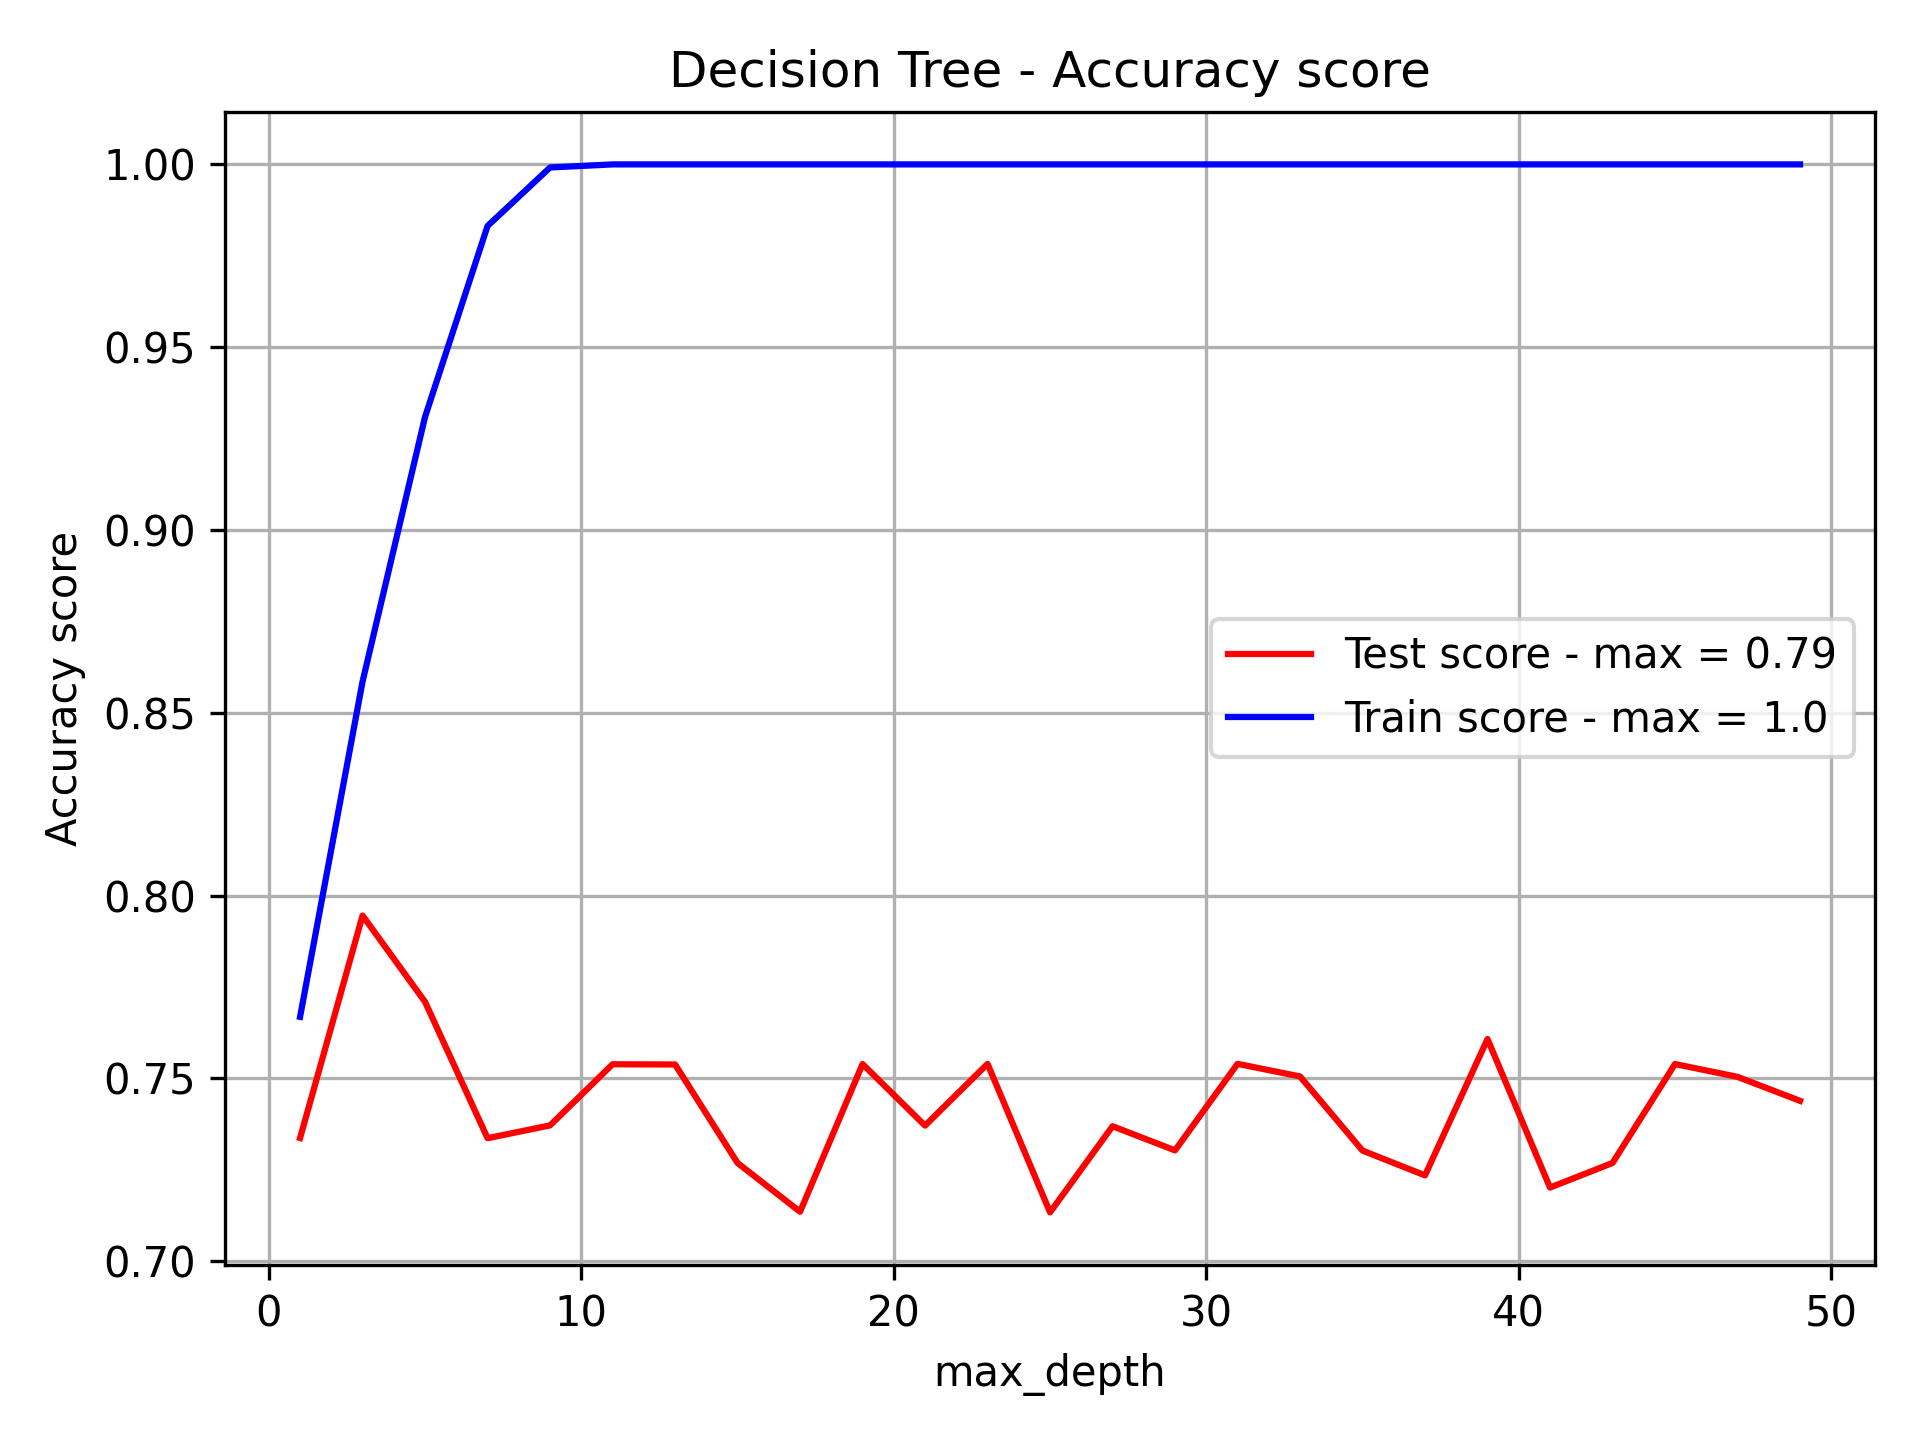
\includegraphics[width=\columnwidth]{dt_max_depth_vs_accuracy.png}
    \caption{Figure 7 plots the accuracy for both the training and test set as a function of $max\_depth$.}
    \label{fig:7}
\end{figure}\\
From studying figure \ref{fig:7}, we can clearly see that the decision tree overfits to the training set. As the $\verb"max_depth"$ increases, the accuracy on the training set converges at a perfect score of $1.0$. While for the test set, the accuracy score becomes worse and generally hovers slightly below $0.75$. The accuracy for the test set follows the training set until $\verb"max_depth"$ $> 3$ but worsens due to overfitting. \\
\\
Next we tune other relevant parameters to see if the performance improves. Doing a grid search of the parameters $\verb"max_depth"$, $\verb"min_samples_split"$, $\verb"min_samples_leaf"$ and $\verb"splitter"$ results in table \ref{tab:2}.
\begin{table}[h]
    \centering
    \caption{Table sorted by mean test score achieved when doing a grid search of parameters with decision tree. Number of folds $k = 5$. Top 15 results.}
    \label{tab:2}
    \begin{tabular}{|P{0.7cm}|P{0.9cm}|P{1.2cm}|P{1.2cm}|P{1.1cm}|P{0.8cm}|}
    \hline
    \cellcolor{gray!25} \textbf{rank} & \cellcolor{gray!25} \textbf{max depth} & \cellcolor{gray!25} \textbf{min\newline samples split} & \cellcolor{gray!25} \textbf{min\newline samples leaf} & \cellcolor{gray!25} \textbf{splitter} &  \cellcolor{gray!25} \textbf{mean test score} \\
    \hline
    \hline
    1 & 50 & 2 & 0.1 & random & 0.80 \\
    \hline
    2 & 10 & 4 & 0.2 & random & 0.80 \\
    \hline
    2 & 100 & 4 & 0.2 & random & 0.80 \\
    \hline
    4 & 5 & 5 & 1 & random & 0.80 \\
    \hline
    5 & 40 & 5 & 0.4 & random & 0.79 \\
    \hline
    5 & 100 & 5 & 0.1 & random & 0.79 \\
    \hline
    7 & None & 5 & 0.1 & random & 0.79 \\
    \hline
    8 & 50 & 5 & 0.3 & random & 0.78 \\
    \hline
    8 & 20 & 5 & 0.3 & random & 0.78 \\
    \hline
    8 & 100 & 2 & 0.2 & random & 0.78 \\
    \hline
    8 & 40 & 3 & 0.3 & random & 0.78 \\
    \hline
    8 & 20 & 2 & 0.3 & random & 0.78 \\
    \hline
    13 & 20 & 2 & 0.1 & random & 0.78 \\
    \hline
    14 & 100 & 2 & 0.4 & random & 0.78 \\
    \hline
    14 & 40 & 4 & 0.4 & random & 0.78 \\
    \hline
    \end{tabular}
\end{table}\\
The accuracy on the test set only improved by $0.01$ when using the parameters in the first entry in table \ref{tab:2}. Therefore $0.8$, may be the limit on the accuracy we can achieve with decision trees. Suprisingly, using a \textit{random} splitting strategy for the features at each internal node instead of the \textit{best} strategy resulted in the highest accuracy overall. The introduction of randomness to slightly reduce overfitting is likely the reason for this. Still, there is not a large difference in the mean test score.\\
\\
Figure \ref{fig:8a} and \ref{fig:8b} plots the confusion matrix and the ROC curve respectively using the parameters for the model performing best on an untouched test set.
\begin{figure}[ht!]
    \centering
    \begin{subfigure}[b]{\columnwidth}
        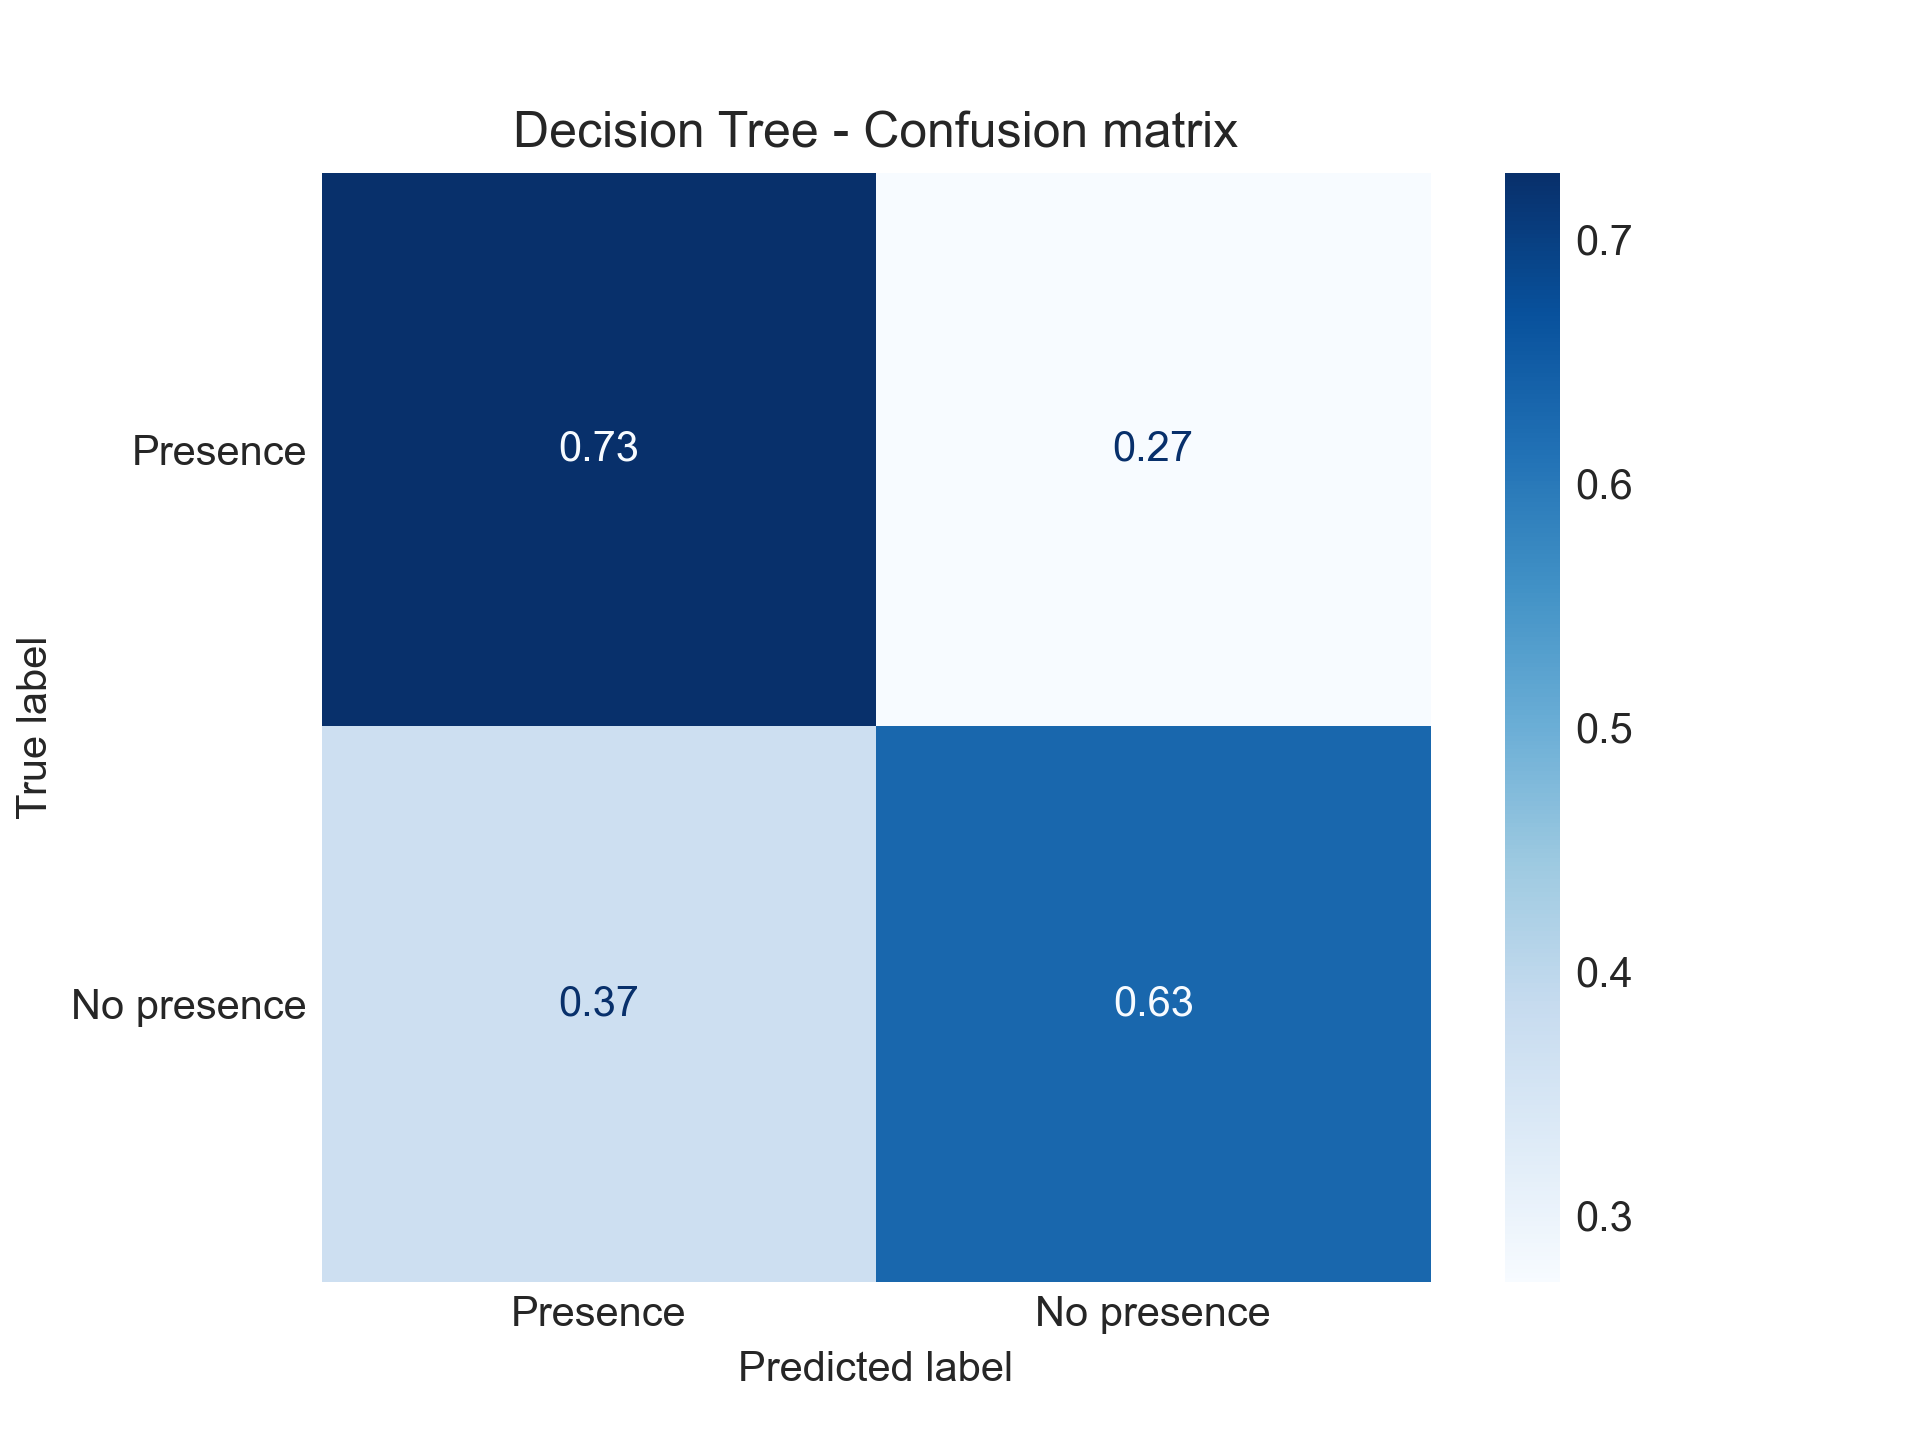
\includegraphics[width=\columnwidth]{dt_confusion_matrix_max_depth=50_min_samples_leaf=0.1_min_samples_split=2_splitter=random.png}
        \caption{Confusion matrix with a decision tree using the parameters max depth=50, min samples leaf=0.1, min samples split=2 and splitter=random.}
        \label{fig:8a}
    \end{subfigure}
    
    \begin{subfigure}[b]{\columnwidth}
        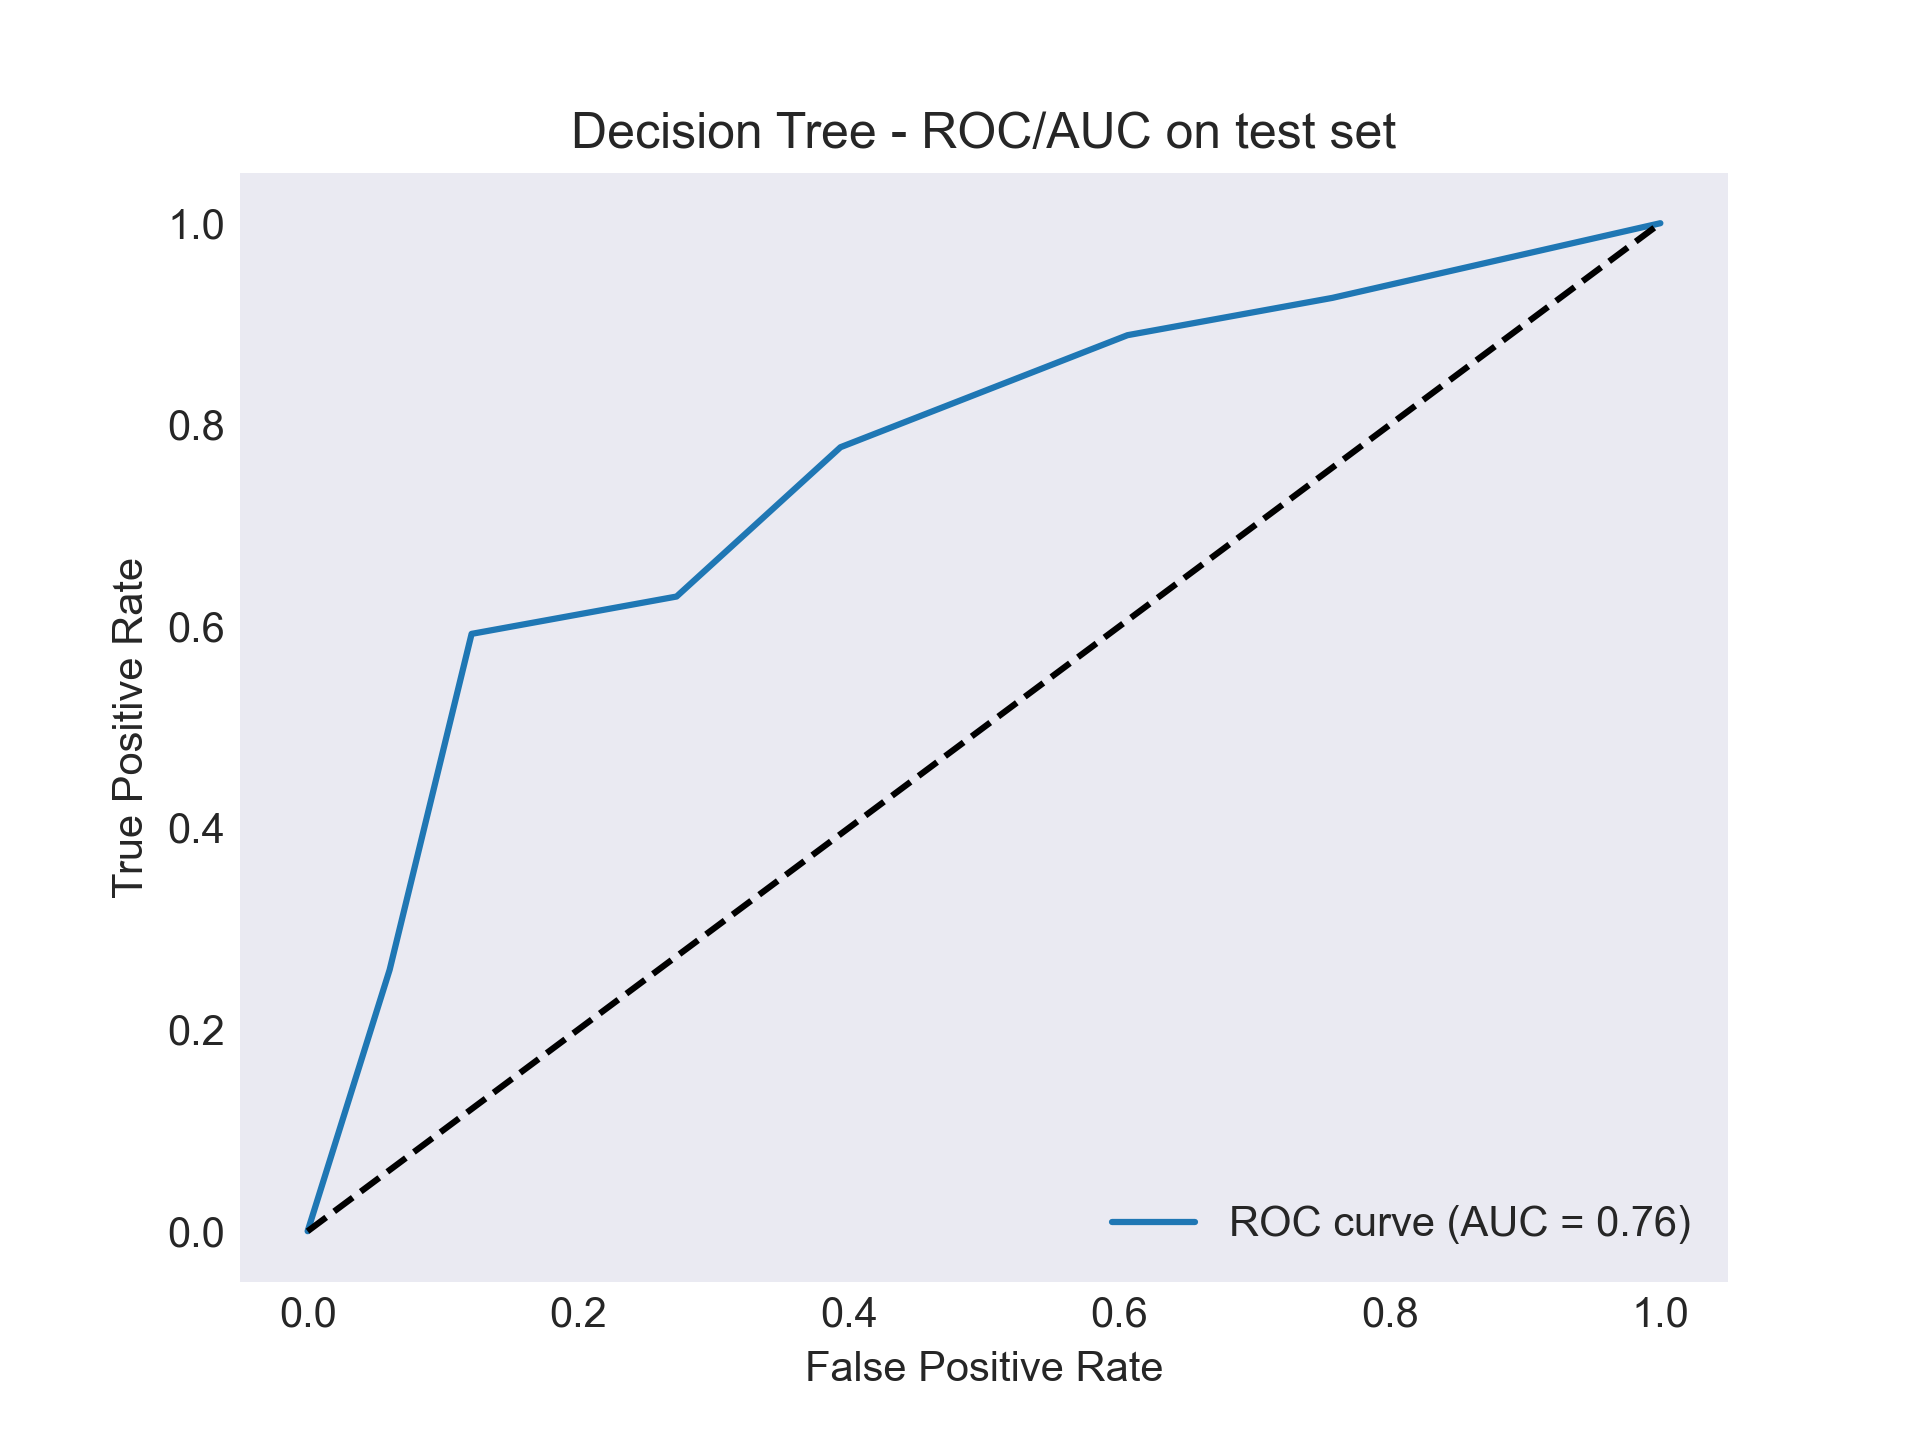
\includegraphics[width=\columnwidth]{dt_roc_curve_max_depth=50_min_samples_leaf=0.1_min_samples_split=2_splitter=random.png}
        \caption{ROC curve with a decision tree using the parameters max depth=50, min samples leaf=0.1, min samples split=2 and splitter=random.}
        \label{fig:8b}
    \end{subfigure}
    \caption{8(a) plots the confusion matrix using a decision tree on an untouched test set. 8(b) plots the ROC curve and shows the AUC using a decision tree on an untouched test set. For both figures, the parameters achieving the best test score in table \ref{tab:2} is used.}
\end{figure}\\
\\
Studying figure \ref{fig:8a}, we see that $27\%$ of the instances with heart disease presence was misclassified as having no heart disease presence. This is not an acceptable performance due to the consequences of misclassification. For the instances with no heart disease presence the misclassification percentage is even worse at $37\%$, and while the consequences of incorrectly classifying no presence are lower the performance of the decision tree is quite poor.\\
\\
Studying the ROC curve in figure \ref{fig:8b}, we can see that the TPR and FPR increases at a similar rate together for a higher TPR. This means that using a decision tree with the "optimal" parameters found is only slightly better than random guessing. Ideally we would like a high TPR and a low FPR, which means the model is more capable of distinguishing between heart disease presence and no heart disease presence. The area under the curve is equal to AUC $= 0.76$, which is not terrible but it is not good either considering the problem the model is applied to.\\
\\
Next we apply random forests to the dataset. The results of a grid search of similar parameters is provided in table \ref{tab:3}.
\begin{table}[h]
    \centering
    \caption{Table sorted by mean test score achieved when doing a grid search of parameters with random forest. Number of folds $k = 5$. Top 15 results.}
    \label{tab:3}
    \begin{tabular}{|P{0.7cm}|P{1.3cm}|P{1.2cm}|P{0.85cm}|P{1.2cm}|P{0.8cm}|}
    \hline
    \cellcolor{gray!25} \textbf{rank} & \cellcolor{gray!25} \textbf{n estimators} & \cellcolor{gray!25} \textbf{max\newline features} & \cellcolor{gray!25} \textbf{max\newline depth} & \cellcolor{gray!25} \textbf{min \newline samples leaf} & \cellcolor{gray!25} \textbf{mean test score} \\
    \hline
    \hline
    1 & 500 & log2 & 10 & 0.2 & 0.85 \\
    \hline
    1 & 250 & log2 & 40 & 0.2 & 0.85 \\
    \hline
    1 & 1000 & sqrt & 40 & 0.2 & 0.85 \\
    \hline
    4 & 100 & sqrt &  3 & 0.2 & 0.85 \\
    \hline
    5 & 250 & sqrt &  5 & 0.2 & 0.85 \\
    \hline
    5 & 250 & log2 & 20 & 0.2 & 0.85 \\
    \hline
    5 & 500 & log2 &  5 & 0.2 & 0.85 \\
    \hline
    5 & 2000 & sqrt & 30 & 0.2 & 0.85 \\
    \hline
    5 & 750 & sqrt &  3 & 0.2 & 0.85 \\
    \hline
    5 & 50 & sqrt & 10 & 0.2 & 0.85 \\
    \hline
    5 & 1000 & log2 & 30 & 0.2 & 0.85 \\
    \hline
    12 & 750 & log2 & None & 0.2 & 0.85 \\
    \hline
    12 & 250 & sqrt & None & 0.2 & 0.85 \\
    \hline
    12 & 1000 & sqrt & 20 & 0.2 & 0.85 \\
    \hline
    15 & 50 & log2 & 20 & 0.1 & 0.85 \\
    \hline
    \end{tabular}
\end{table}\\
From table \ref{tab:3} we see that random forests for all parameters achieve an accuracy of $0.85$, while compared to table \ref{tab:2} the accuracy score varies more for different parameters. This result is consistent with what we stated earlier, that random forests reduces the variance by creating multiple decision trees with different and fewer features. This means the model is less likely to overfit to the training set and thus performs better on an untouched test set. Using random forests allows us spend less time tuning, but the training of the model takes more time.\\
\\
Generally we see that $\verb"min_samples_leaf"$ $= 0.2$ is the optimal value. In addition, the entries in table \ref{tab:3} is approximately evenly split between using \textit{sqrt} and \textit{log}$_{2}$ for $\verb"max_features"$. When presenting random forests earlier, it was mentioned that $m \approx \sqrt{p}$ is usually the standard but the results show that $m \approx log_{2}(p)$ is a perfectly valid option. During the grid search, $m = p$ was also tested but it does not show up in table \ref{tab:3} due to the model performing better not considering all features when constructing trees. \\
\\
Also noticeable is that random forests generally performs better for a lower $\verb"max_depth"$ compared to decision trees. Furthermore, increasing $\verb"n_estimators"$, i.e. the number of decision trees constructed, has diminishing returns once at a certain number. From table \ref{tab:3}, the  upper bound on the number of trees needed is around 250 and more trees than this is not likely to improve the accuracy. To test this, the accuracy on the test set is plotted as a function of $\verb"n_estimators"$ in figure \ref{fig:9}.
\begin{figure}[ht]
    \centering
    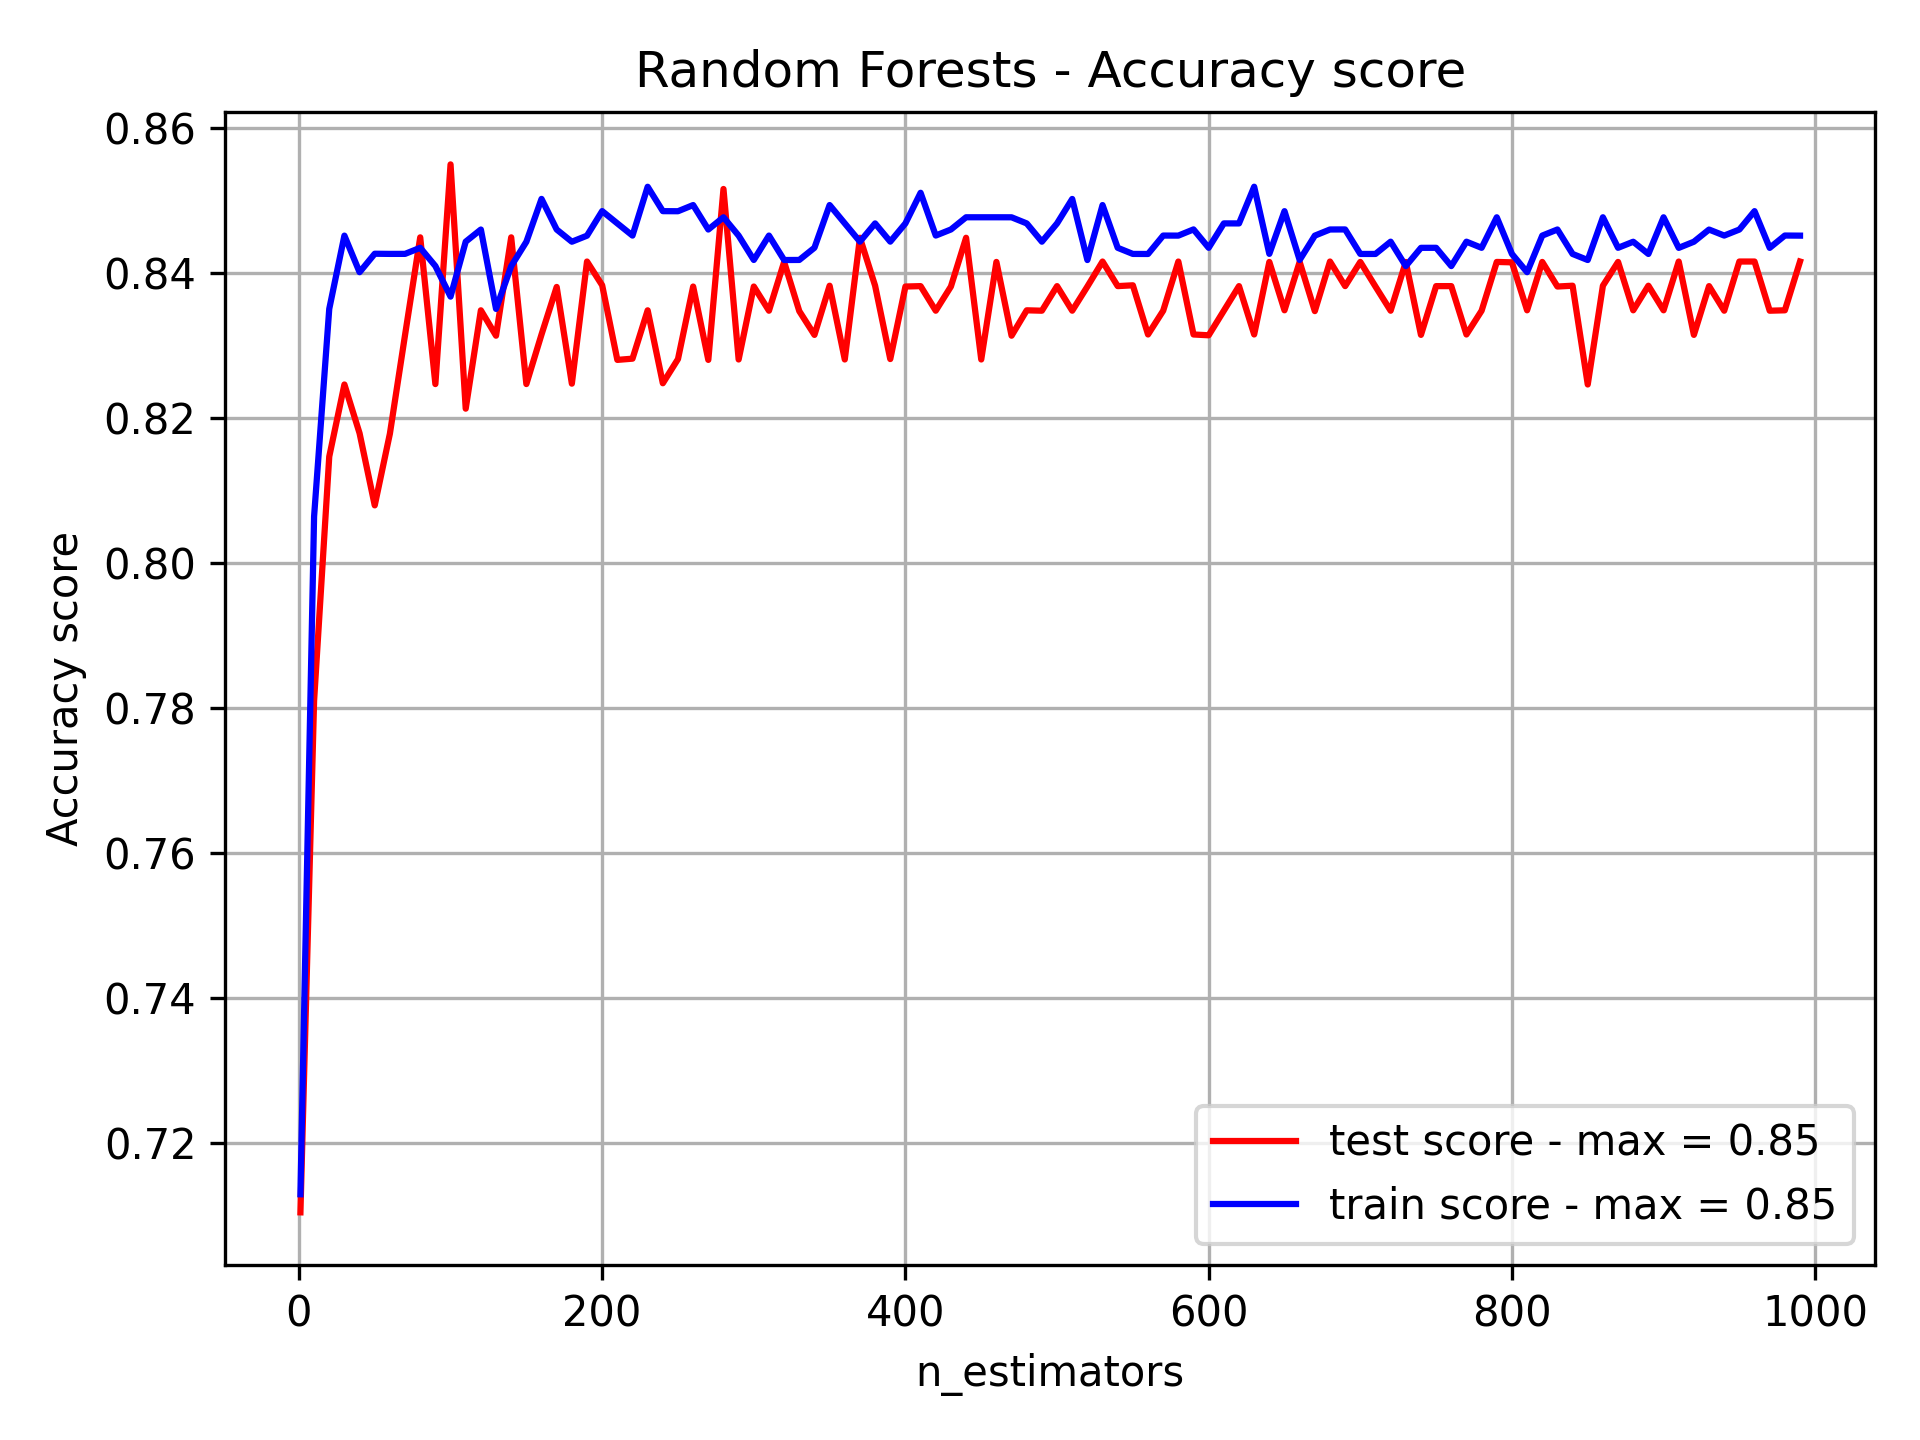
\includegraphics[width=\columnwidth]{rf_n_estimators_vs_accuracy.png}
    \caption{Figure 9 plots the accuracy score for both the training and test set as a function of $n\_estimators$, with the random forest using the parameters max features = log2, max depth = 10 and min samples leaf = 0.2}
    \label{fig:9}
\end{figure}\\
Studying figure \ref{fig:9}, we see that the accuracy on both the test set and training set converges for a relatively low number of trees constructed. The accuracy seems to converge at around $\verb"n_estimators"$ $\approx 100$.
\begin{figure}[ht!]
    \centering
    \begin{subfigure}[b]{\columnwidth}
        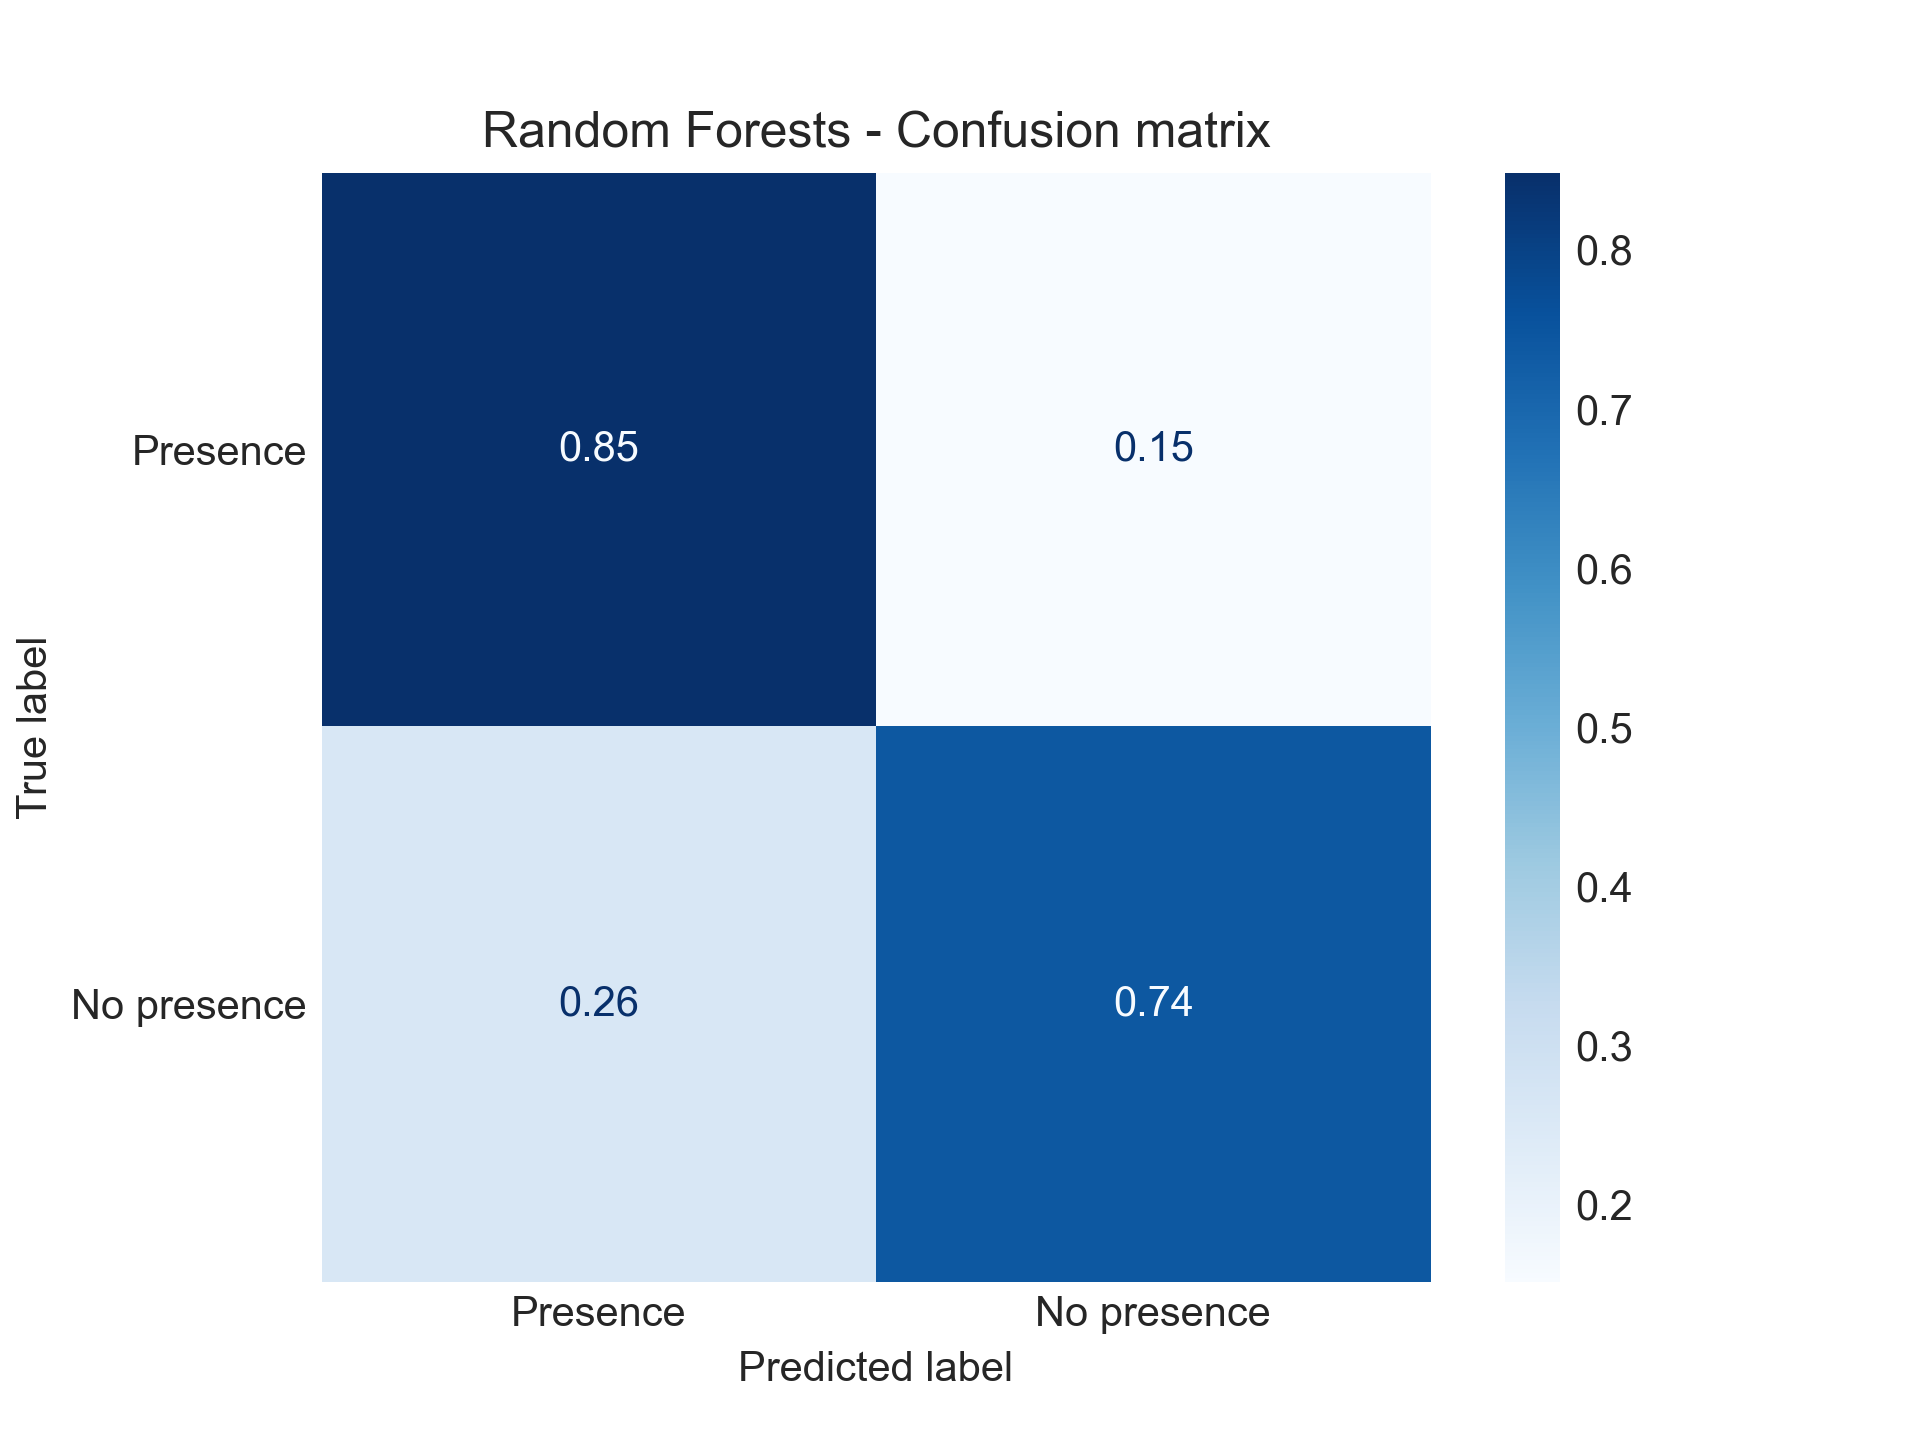
\includegraphics[width=\columnwidth]{rf_confusion_matrix_max_depth=10_max_features=log2_min_samples_leaf=0.2_n_estimators=500.png}
        \caption{Confusion matrix with random forest using the parameters max depth=10, max features=log2, min samples leaf=0.2 and n estimators=500.}
        \label{fig:10a}
    \end{subfigure}
    
    \begin{subfigure}[b]{\columnwidth}
        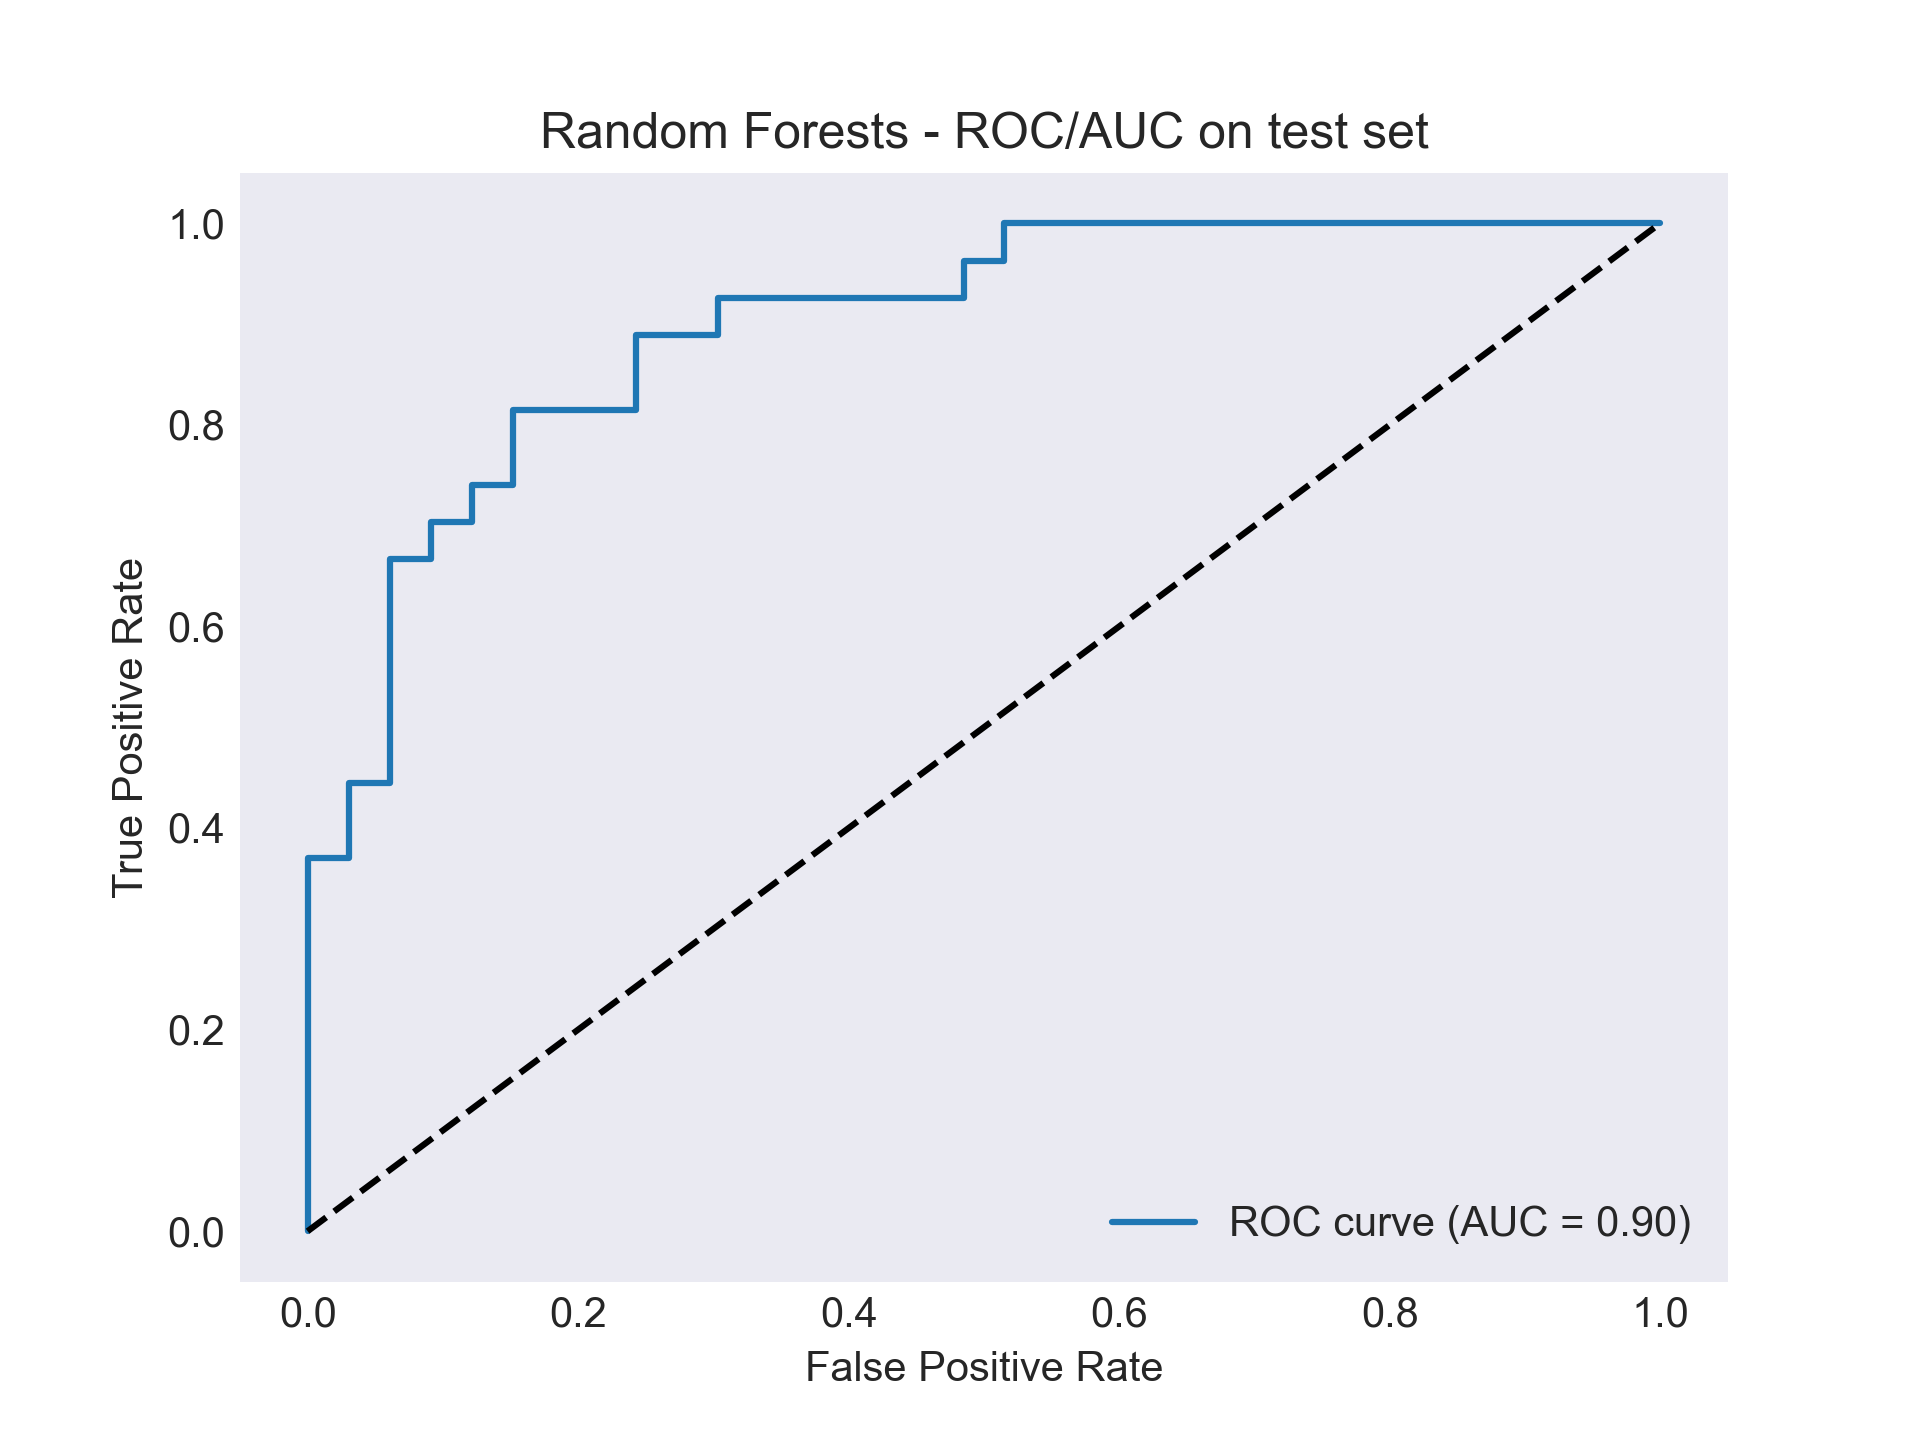
\includegraphics[width=\columnwidth]{rf_roc_curve_max_depth=10_max_features=log2_min_samples_leaf=0.2_n_estimators=500.png}
        \caption{ROC curve with random forest using the parameters max depth=10, max features=log2, min samples leaf=0.2 and n estimators=500.}
        \label{fig:10b}
    \end{subfigure}
    \caption{10(a) plots the confusion matrix using random forest on an untouched test set. 10(b) plots the ROC curve and shows the AUC using random forest on an untouched test set. For both figures, the parameters achieving the best test score in table \ref{tab:3} is used.}
    \label{fig:10}
\end{figure}
The varying accuracy score is due to the randomness of introduced by the resampling technique. Also noticeable is that there is not a substantial difference between the accuracy on the training set and the test set, which again demonstrates the ability of random forests to not overfit as much as decision trees.
\\
\\
While random forests achieves a maximum accuracy of $0.85$ in table \ref{tab:3}, only $0.5$ more than decision trees, it is still a  substantial improvement. The difference becomes more apparent when studying the confusion matrix and ROC curve in figure \ref{fig:10}.\\
\\
From the confusion matrix in figure \ref{fig:10a}, the misclassification ratio of instances with heart disease presence is almost halved compared to decision trees in \ref{fig:8a}. This is a substantial improvement, which was expected beforehand due to random forests being more general and not overfitted to the training set. However there is room for improvement, especially the misclassification of instances with no heart disease where $1/4$ of the instances in the test set is incorrectly classified. \\
\\
The ROC curve in figure \ref{fig:10b} also shows substantial improvements over decision trees, where the true positive rate (TPR) is larger for lower false positive rate (FPR). Using random forests outperforms decision trees which are only slightly perform better than random guessing. Furthermore, the AUC score for random forests is equal to AUC $= 0.90$, greater than $0.76$ with decison trees which confirms that random forests perform better than decision tress on this particular classification problem.\\
\\
Finally, we study the performance of boosting methods on the classification problem. Starting with AdaBoost, table \ref{tab:4} contains the top 15 results when doing a grid search of the most relevant parameters.\\
\\ 
AdaBoost is able to achieve the same maximum accuracy of $0.85$ on an untocuhed dataset as random forests. Generally AdaBoost performs best for a $\verb"learning_rate"$ $< 0.1$, and also there seems to be a correlation between the number of "stumps" constructed and the learning rate. The larger the number of "stumps" constructed is, the lower the learning rate needs to be for most of the entries in table \ref{tab:4}. Whereas for a smaller number of "stumps", a larger learning rate is needed. When using AdaBoost, the number of weak learners needs to be balanced with the learning rate.\\
\begin{table}[h!]
    \centering
    \caption{Table sorted by mean test score achieved when doing a grid search of parameters with AdaBoost. Number of folds $k = 5$. Top 15 results.}
    \label{tab:4}
    \begin{tabular}{|P{0.7cm}|P{1.7cm}|P{1.3cm}|P{1.7cm}|}
    \hline
    \cellcolor{gray!25} \textbf{rank} & \cellcolor{gray!25} \textbf{n \newline estimators} & \cellcolor{gray!25} \textbf{learning rate} & \cellcolor{gray!25} \textbf{mean test score} \\
    \hline
    \hline
    1 & 750 & 0.005 & 0.85 \\
    \hline
    2 & 2000 & 0.001 & 0.85 \\
    \hline
    3 & 1000 & 0.01 & 0.84 \\
    \hline
    3 & 2000 & 0.005 & 0.84 \\
    \hline
    5 & 500 & 0.01 & 0.84 \\
    \hline
    5 & 1000 & 0.005 & 0.84 \\
    \hline
    5 & 1500 & 0.001 & 0.84 \\
    \hline
    8 & 50 & 0.05 & 0.84 \\
    \hline
    8 & 250 & 0.01 & 0.84 \\
    \hline
    8 & 500 & 0.005 & 0.84 \\
    \hline
    11 & 100 & 0.1 & 0.84 \\
    \hline
    11 & 250 & 0.05 & 0.84 \\
    \hline
    11 & 100 & 0.05 & 0.84 \\
    \hline
    14 & 750 & 0.01 & 0.83 \\
    \hline
    14 & 1500 & 0.005 & 0.83 \\
    \hline
    \end{tabular}
\end{table}
\begin{figure}[ht!]
    \centering
    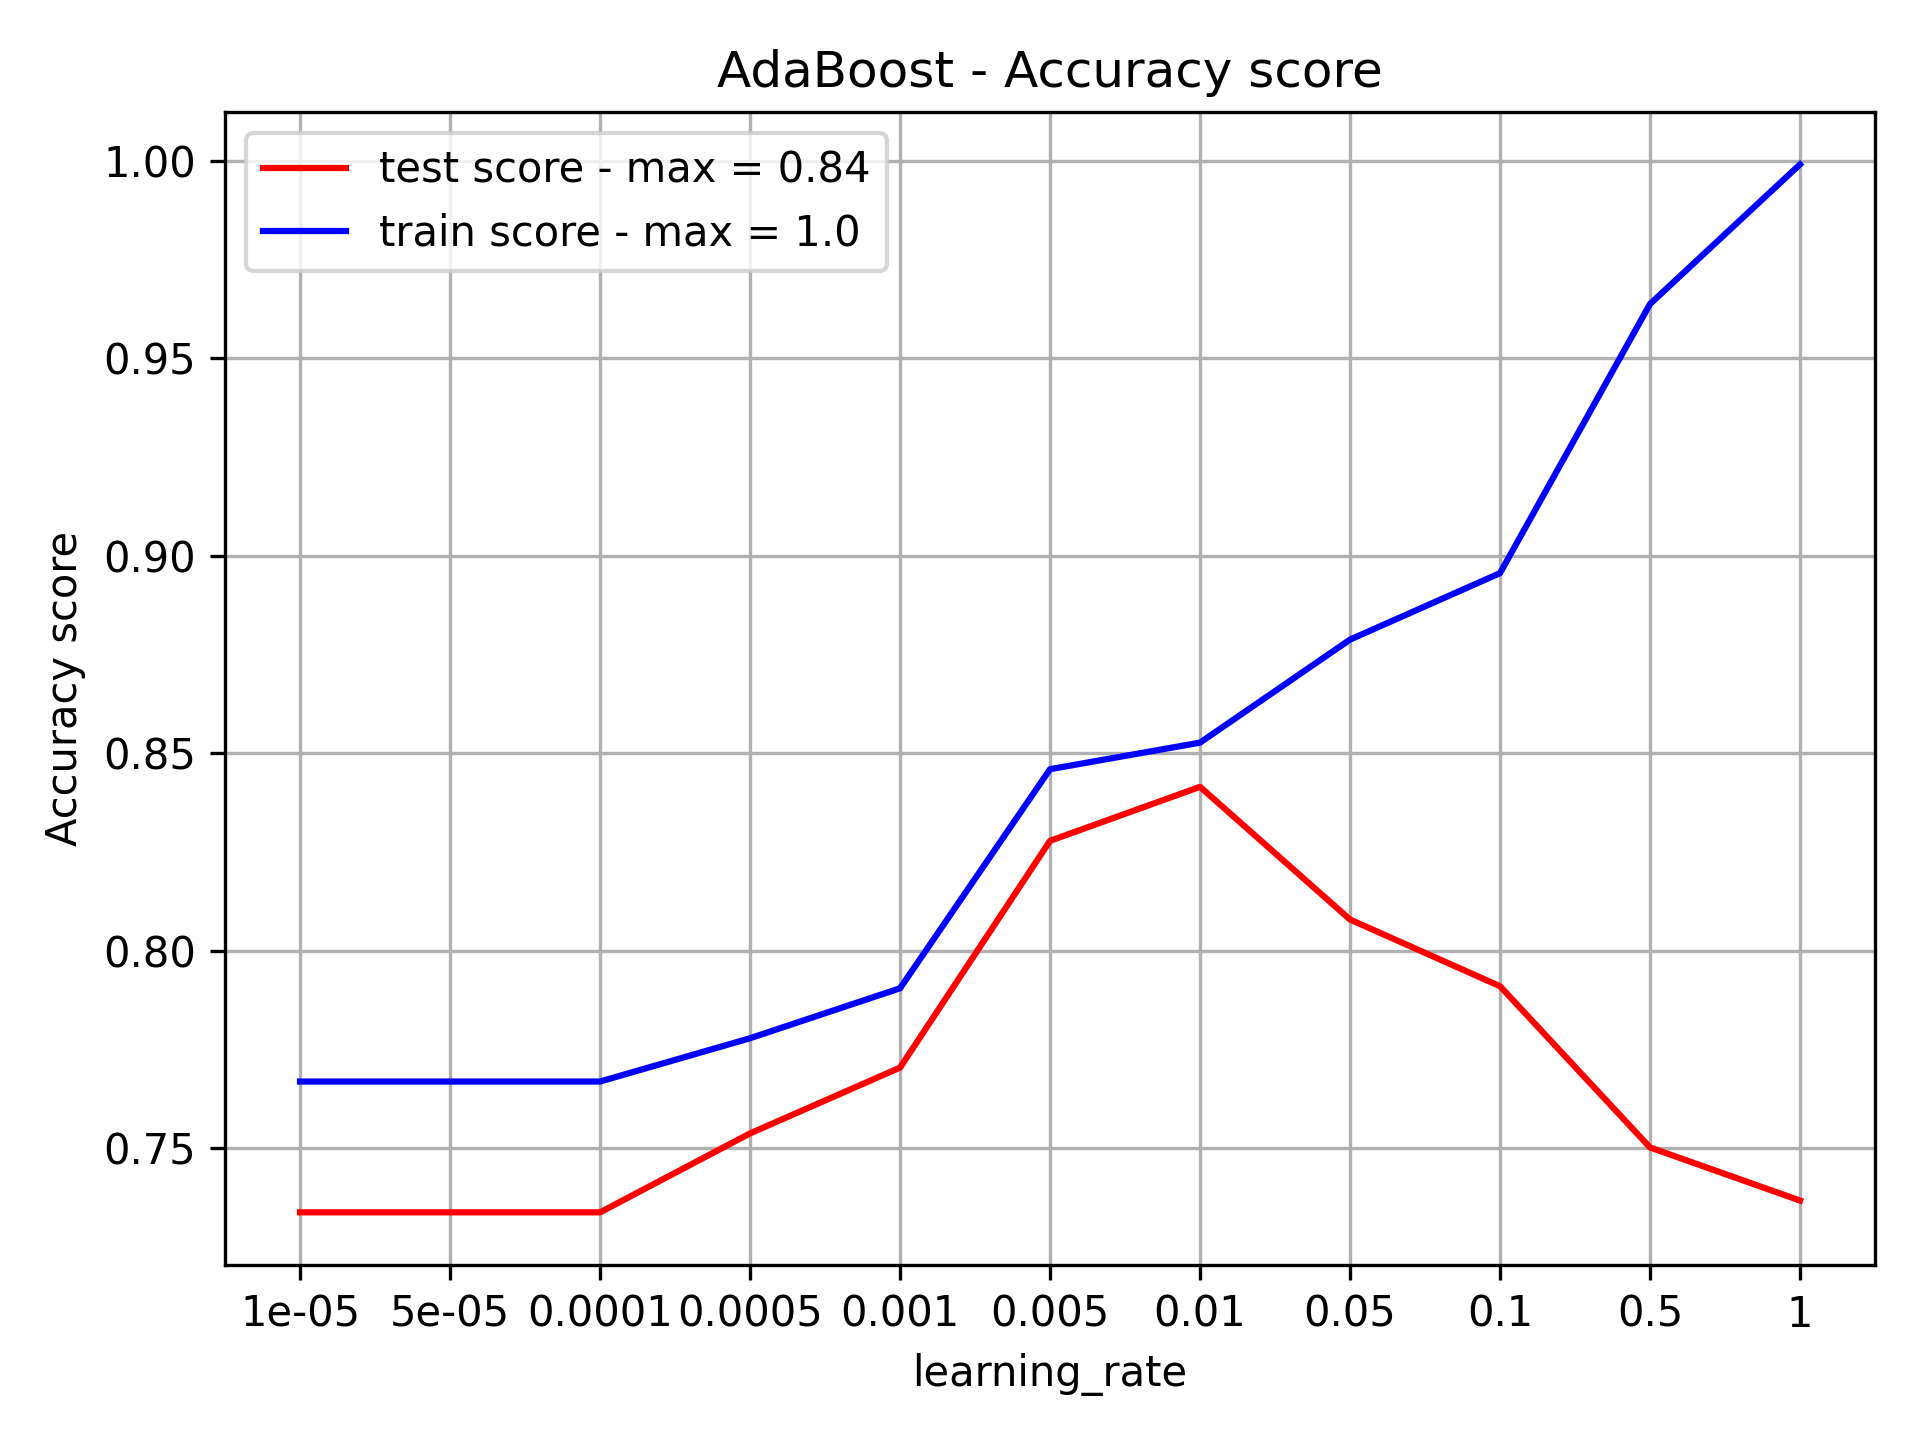
\includegraphics[width=\columnwidth]{abm_learning_rate_vs_accuracy.png}
    \caption{Figure 11 plots the accuracy score for both the training and test set as a function of $learning\_rate$, with the AdaBoost model using the parameters n estimators = 250.}
    \label{fig:11}
\end{figure}\\
The learning rate is used with AdaBoost to shrink the contribution from each weak learner and therefore slow down the "learning" to not overfit. Figure \ref{fig:11} shows that for a $\verb"learning_rate"$ up to approximately $0.1$ plus/minus depending on the number of "stumps" constructed, the accuracy on the training and test set follow each other closely. For a higher $\verb"learning_rate"$ the train score and test score diverges, where the test accuracy worsens and the training accuracy improves. The reason for this is due to overfitting. A larger learning rate causes the model to overfit to the training set, as we see the training accuracy converge at $1.0$ in figure \ref{fig:11}, and is therefore not general enough when applied to the test set.
\begin{figure}[!ht]
    \centering
    \begin{subfigure}[b]{\columnwidth}
        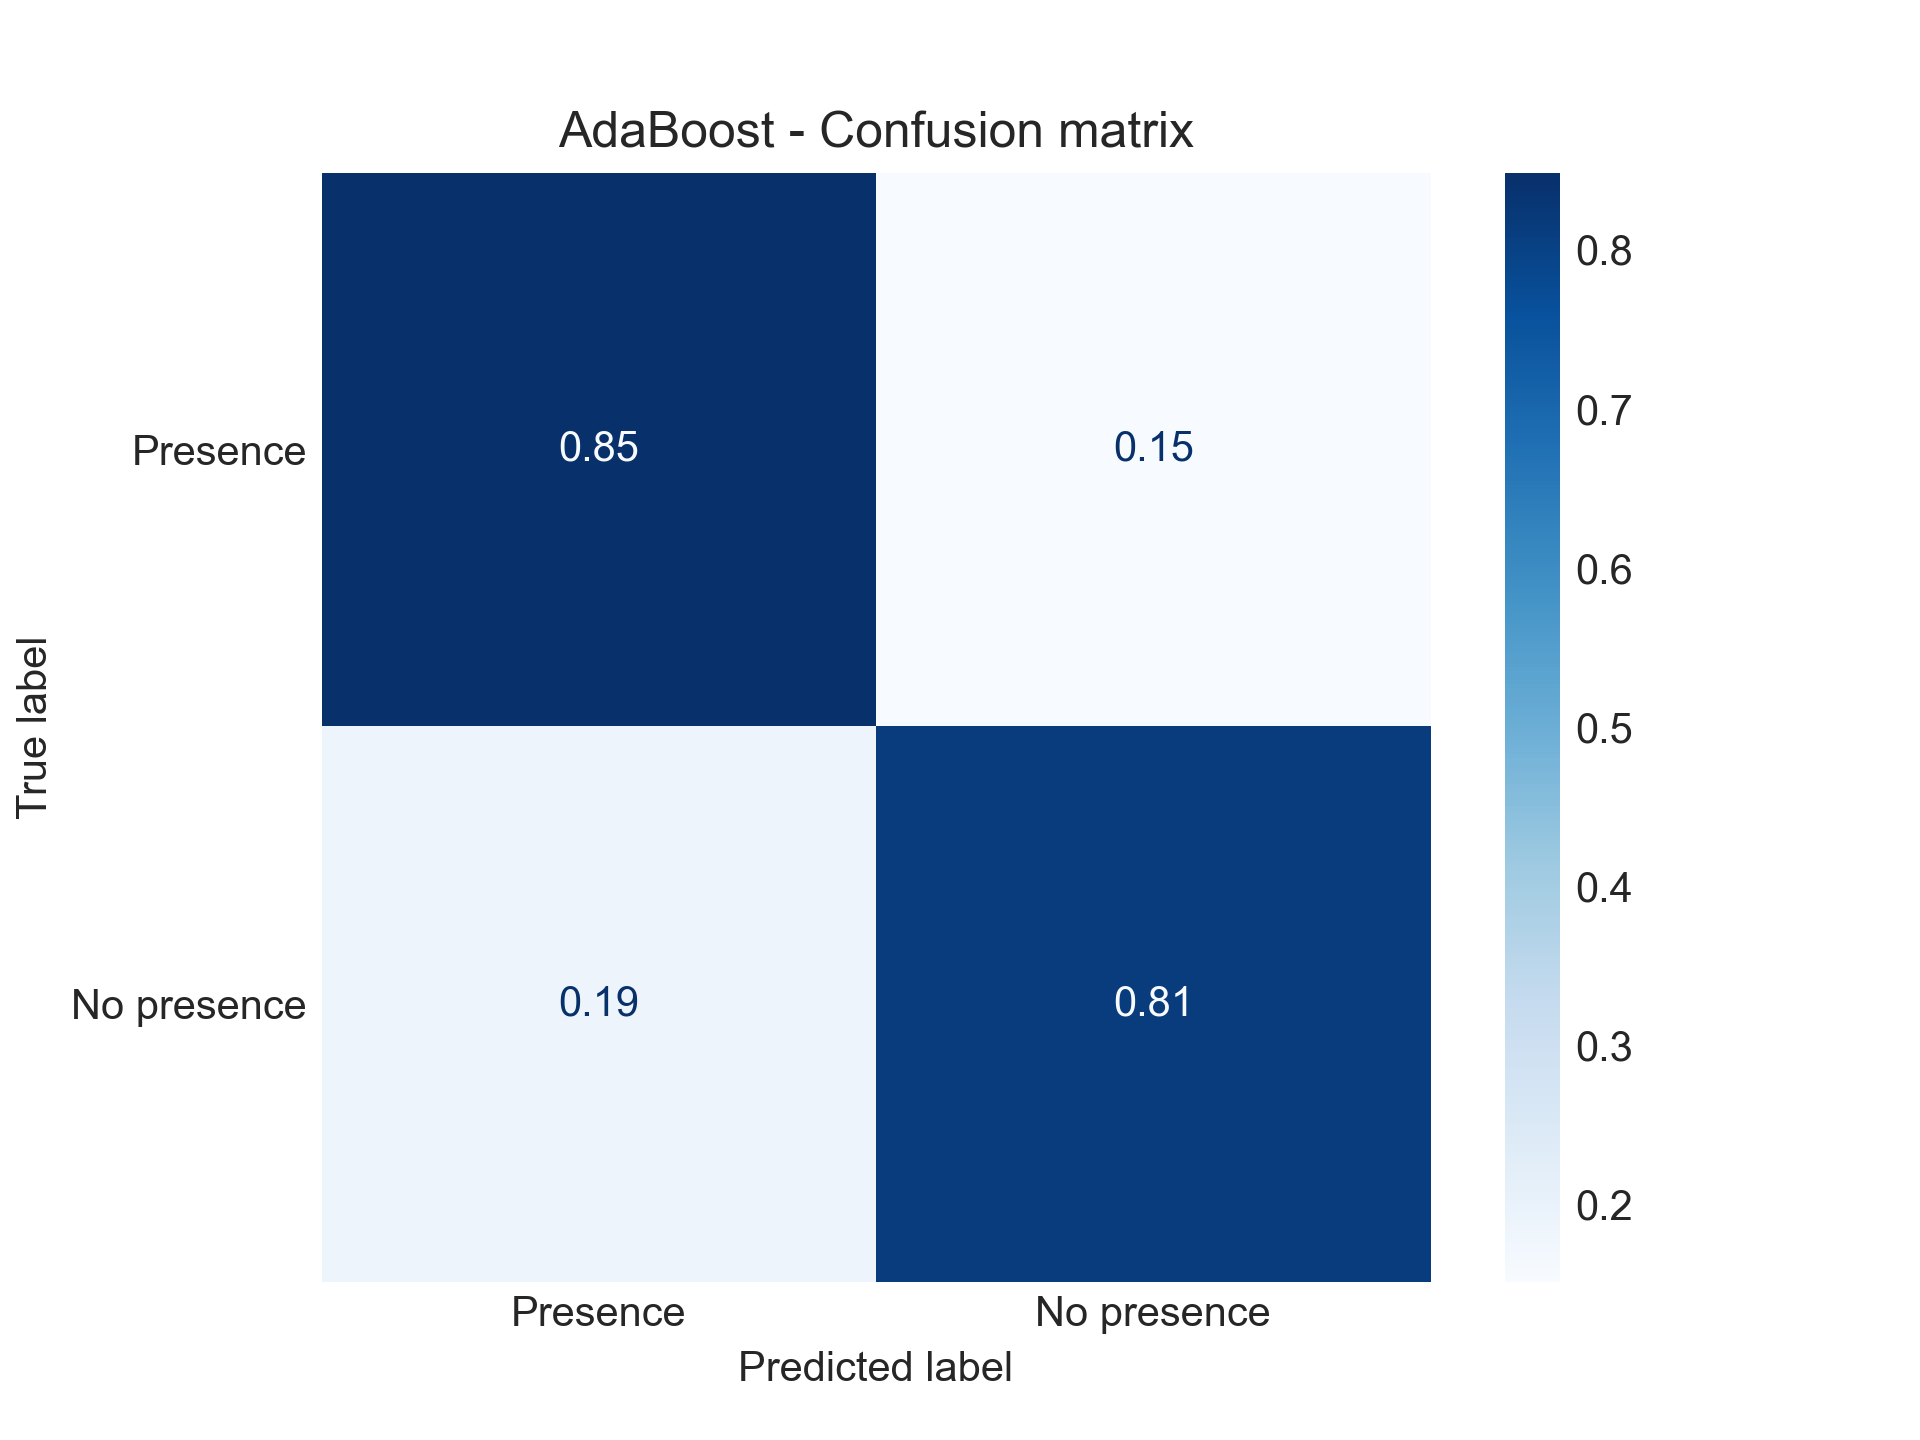
\includegraphics[width=\columnwidth]{abm_confusion_matrix_learning_rate=0.005_n_estimators=750.png}
        \caption{Confusion matrix with AdaBoost using the parameters learning rate = 0.005 and n estimators=750.}
        \label{fig:12a}
    \end{subfigure}
    
    \begin{subfigure}[b]{\columnwidth}
        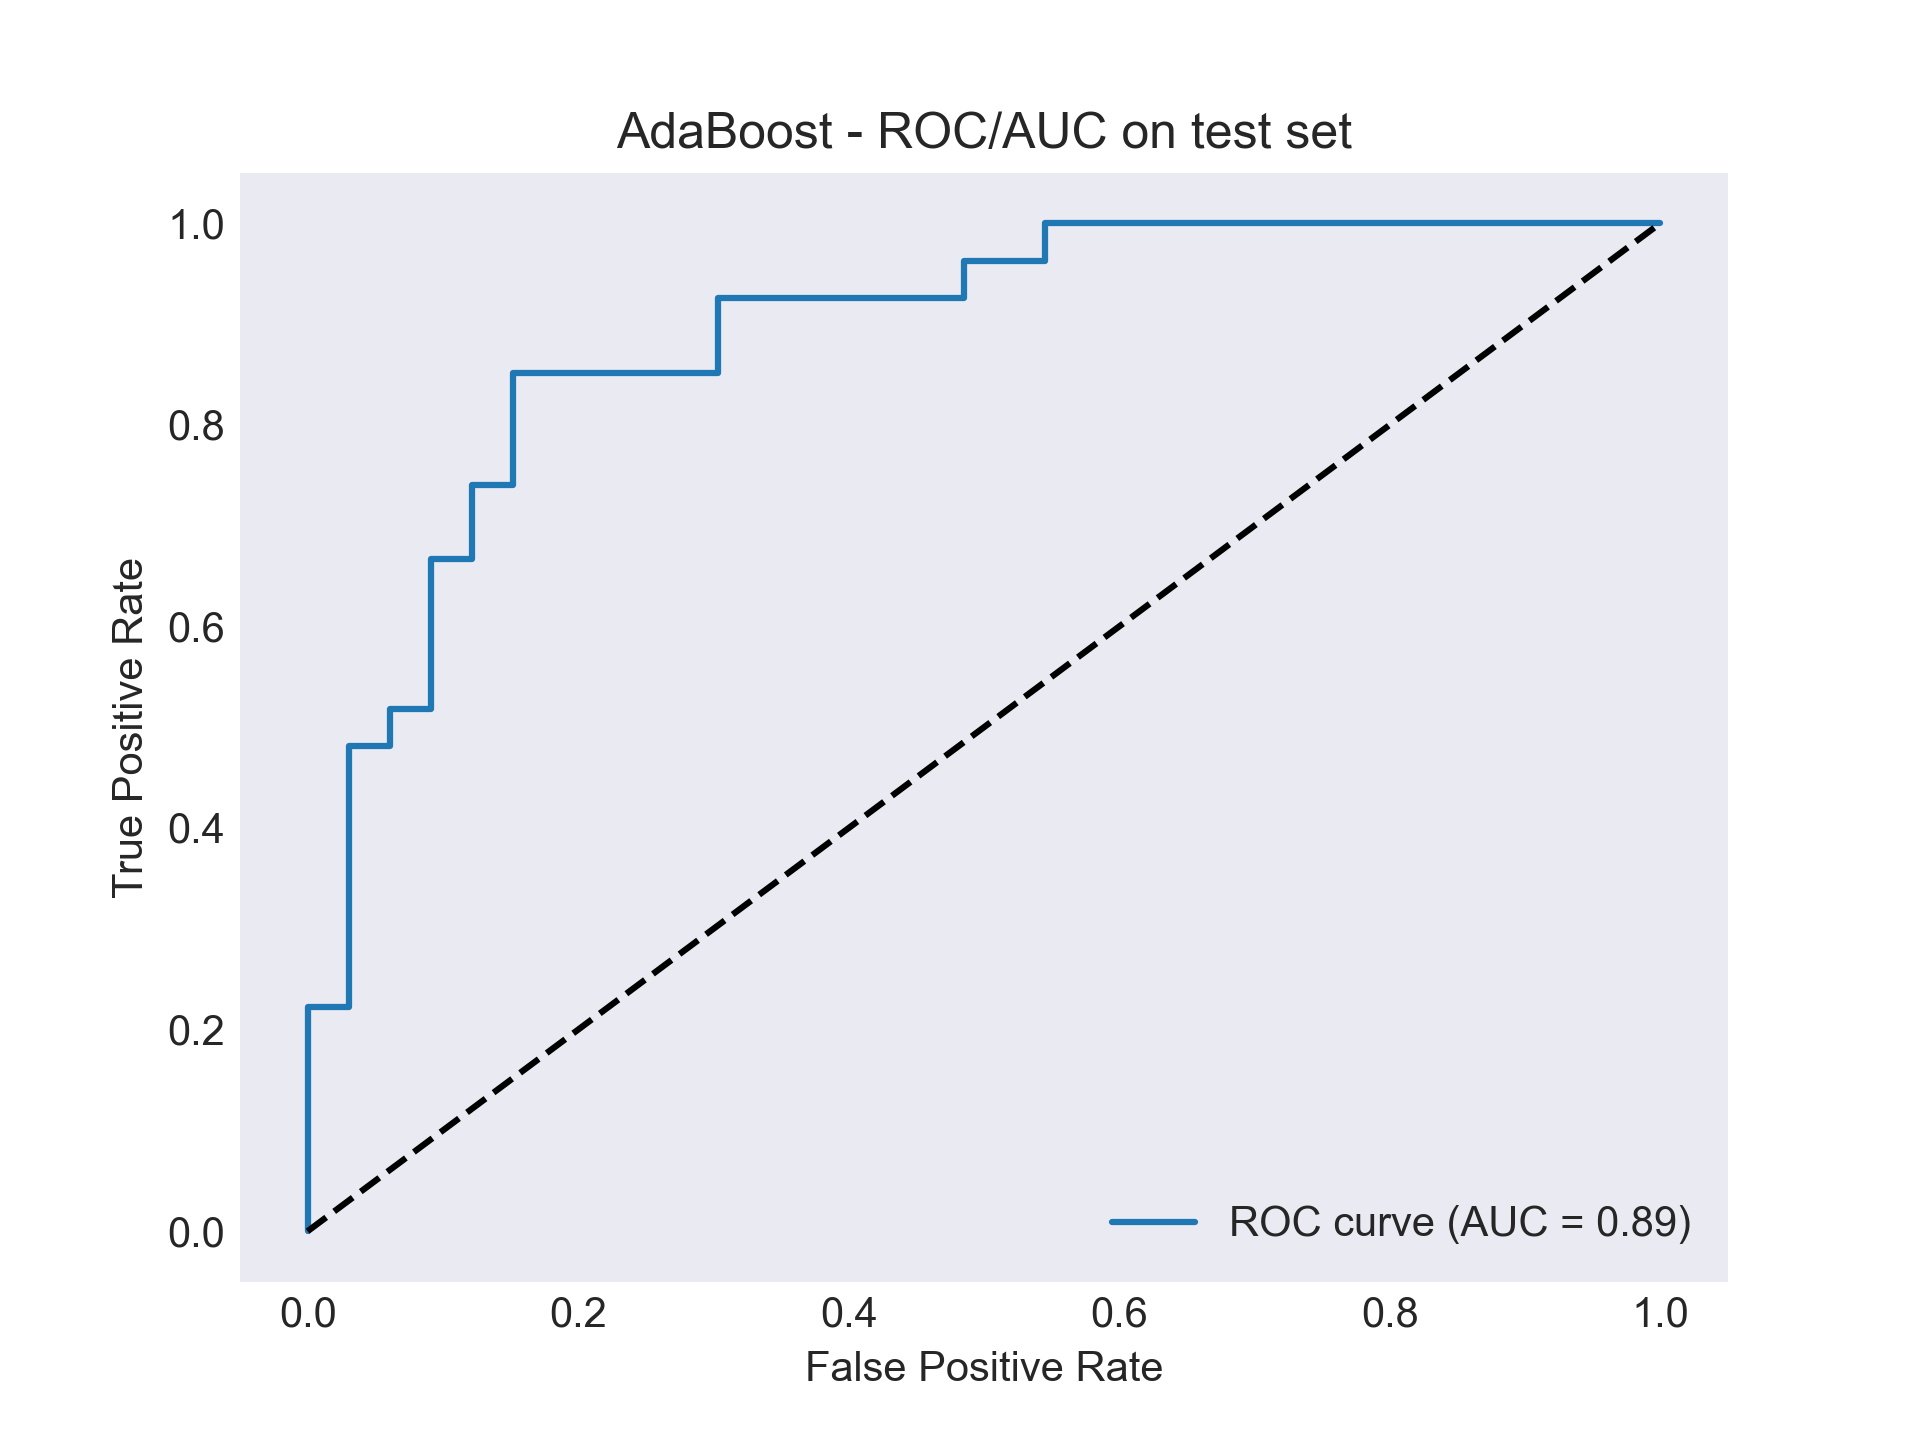
\includegraphics[width=\columnwidth]{abm_roc_curve_learning_rate=0.005_n_estimators=750.png}
        \caption{ROC curve with AdaBoost using the parameters learning rate = 0.005 and n estimators=750.}
        \label{fig:12b}
    \end{subfigure}
    \caption{12(a) plots the confusion matrix using AdaBoost on an untouched test set. 12(b) plots the ROC curve and shows the AUC using AdaBoost on an untouched test set. For both figures, the parameters achieving the best test score in table \ref{tab:4} is used.}
    \label{fig:12}
\end{figure}\\
\\
Figure \ref{fig:12} plots the confusion matrix and ROC curve with an AdaBoost model using the parameters in the first entry of table \ref{tab:4}. Comparing the confusion matrix in figure \ref{fig:12a} for AdaBoost with the confusion matrix in figure \ref{fig:10a}, we can see a substantial improvement when classifying instances with no heart disease presence. AdaBoost is able to achieve a true positive value (TP) and a true negative value (TN) larger than $0.8$.\\
\\
In addition, the ROC curve in figure \ref{fig:12b} is quite similar to the ROC curve for random forests in figure \ref{fig:10b}. Only noticeable difference is that AdaBoost contains a slightly more "optimal" point or threshold on the ROC curve where $TPR \approx 0.85$ and $FPR \approx 0.15$. The performance of AdaBoost and random forests is almost identical, with AdaBoost being slightly better at separating the classes as seen in the confusion matrix.\\
\\
Alternatively, we test gradient boosting which might yield better results. Table \ref{tab:5} contains the top 15 results after performing a grid search of relevant parameters for gradient boosting.
\begin{table}[h!]
    \centering
    \caption{Table sorted by mean test score achieved when doing a grid search of parameters with Gradient Boosting. Number of folds $k = 5$. Top 15 results.}
    \label{tab:5}
    \begin{tabular}{|P{0.7cm}|P{1.22cm}|P{1.25cm}|P{0.8cm}|P{0.9cm}|P{0.9cm}|P{0.8cm}|}
    \hline
    \cellcolor{gray!25} \textbf{rank} & \cellcolor{gray!25} \textbf{n estimators} & \cellcolor{gray!25} \textbf{learning rate} & \cellcolor{gray!25} \textbf{max features} & \cellcolor{gray!25} \textbf{max depth} & \cellcolor{gray!25} \textbf{min samples leaf} & \cellcolor{gray!25} \textbf{mean test score} \\
    \hline
    \hline
    1 & 500 & 0.005 & log2 & 5 & 0.3 & 0.86 \\
    \hline
    1 & 250 & 0.01 & sqrt & None & 0.3 & 0.86 \\
    \hline
    3 & 50 & 0.5 & log2 & 10 & 0.3 & 0.86 \\
    \hline
    4 & 50 & 0.01 & log2 & 20 & 0.2 & 0.85 \\
    \hline
    5 & 500 & 0.005 & log2 & 20 & 0.3 & 0.85 \\
    \hline
    5 & 500 & 0.005 & sqrt & 30 & 0.3 & 0.85 \\
    \hline
    7 & 750 & 0.0005 & log2 & 5 & 0.1 & 0.85 \\
    \hline
    8 & 50 & 0.01 & log2 & 20 & 0.1 & 0.85 \\
    \hline
    9 & 1000 & 0.01 & log2 & None & 0.4 & 0.85 \\
    \hline
    9 & 1000 & 0.01 & log2 & 40 & 0.4 & 0.85 \\
    \hline
    9 & 2000 & 0.005 & sqrt & 20 & 0.4 & 0.85 \\
    \hline
    9 & 1000 & 0.01 & sqrt & 3 & 0.4 & 0.85 \\
    \hline
    9 & 2000 & 0.005 & sqrt & 5 & 0.4 & 0.85 \\
    \hline
    9 & 1000 & 0.01 & sqrt & 40 & 0.4 & 0.85 \\
    \hline
    9 & 100 & 0.05 & sqrt & 20 & 0.4 & 0.85 \\
    \hline
    \end{tabular}
\end{table}
From the results in table \ref{tab:5}, we can see results similar to AdaBoost. Graident boosting on the dataste achieves a maximum accuracy score of $0.86$ on the test set. Only $0.1$ better than AdaBoost and random forests, but more consistent acorss all entries in table \ref{tab:5} comapred to AdaBoost. As was done woth AdaBoost, the accuracy on the test set is plotted as a function of the $\verb"learning_rate"$ in figure \ref{fig:13}.
\begin{figure}[ht]
    \centering
    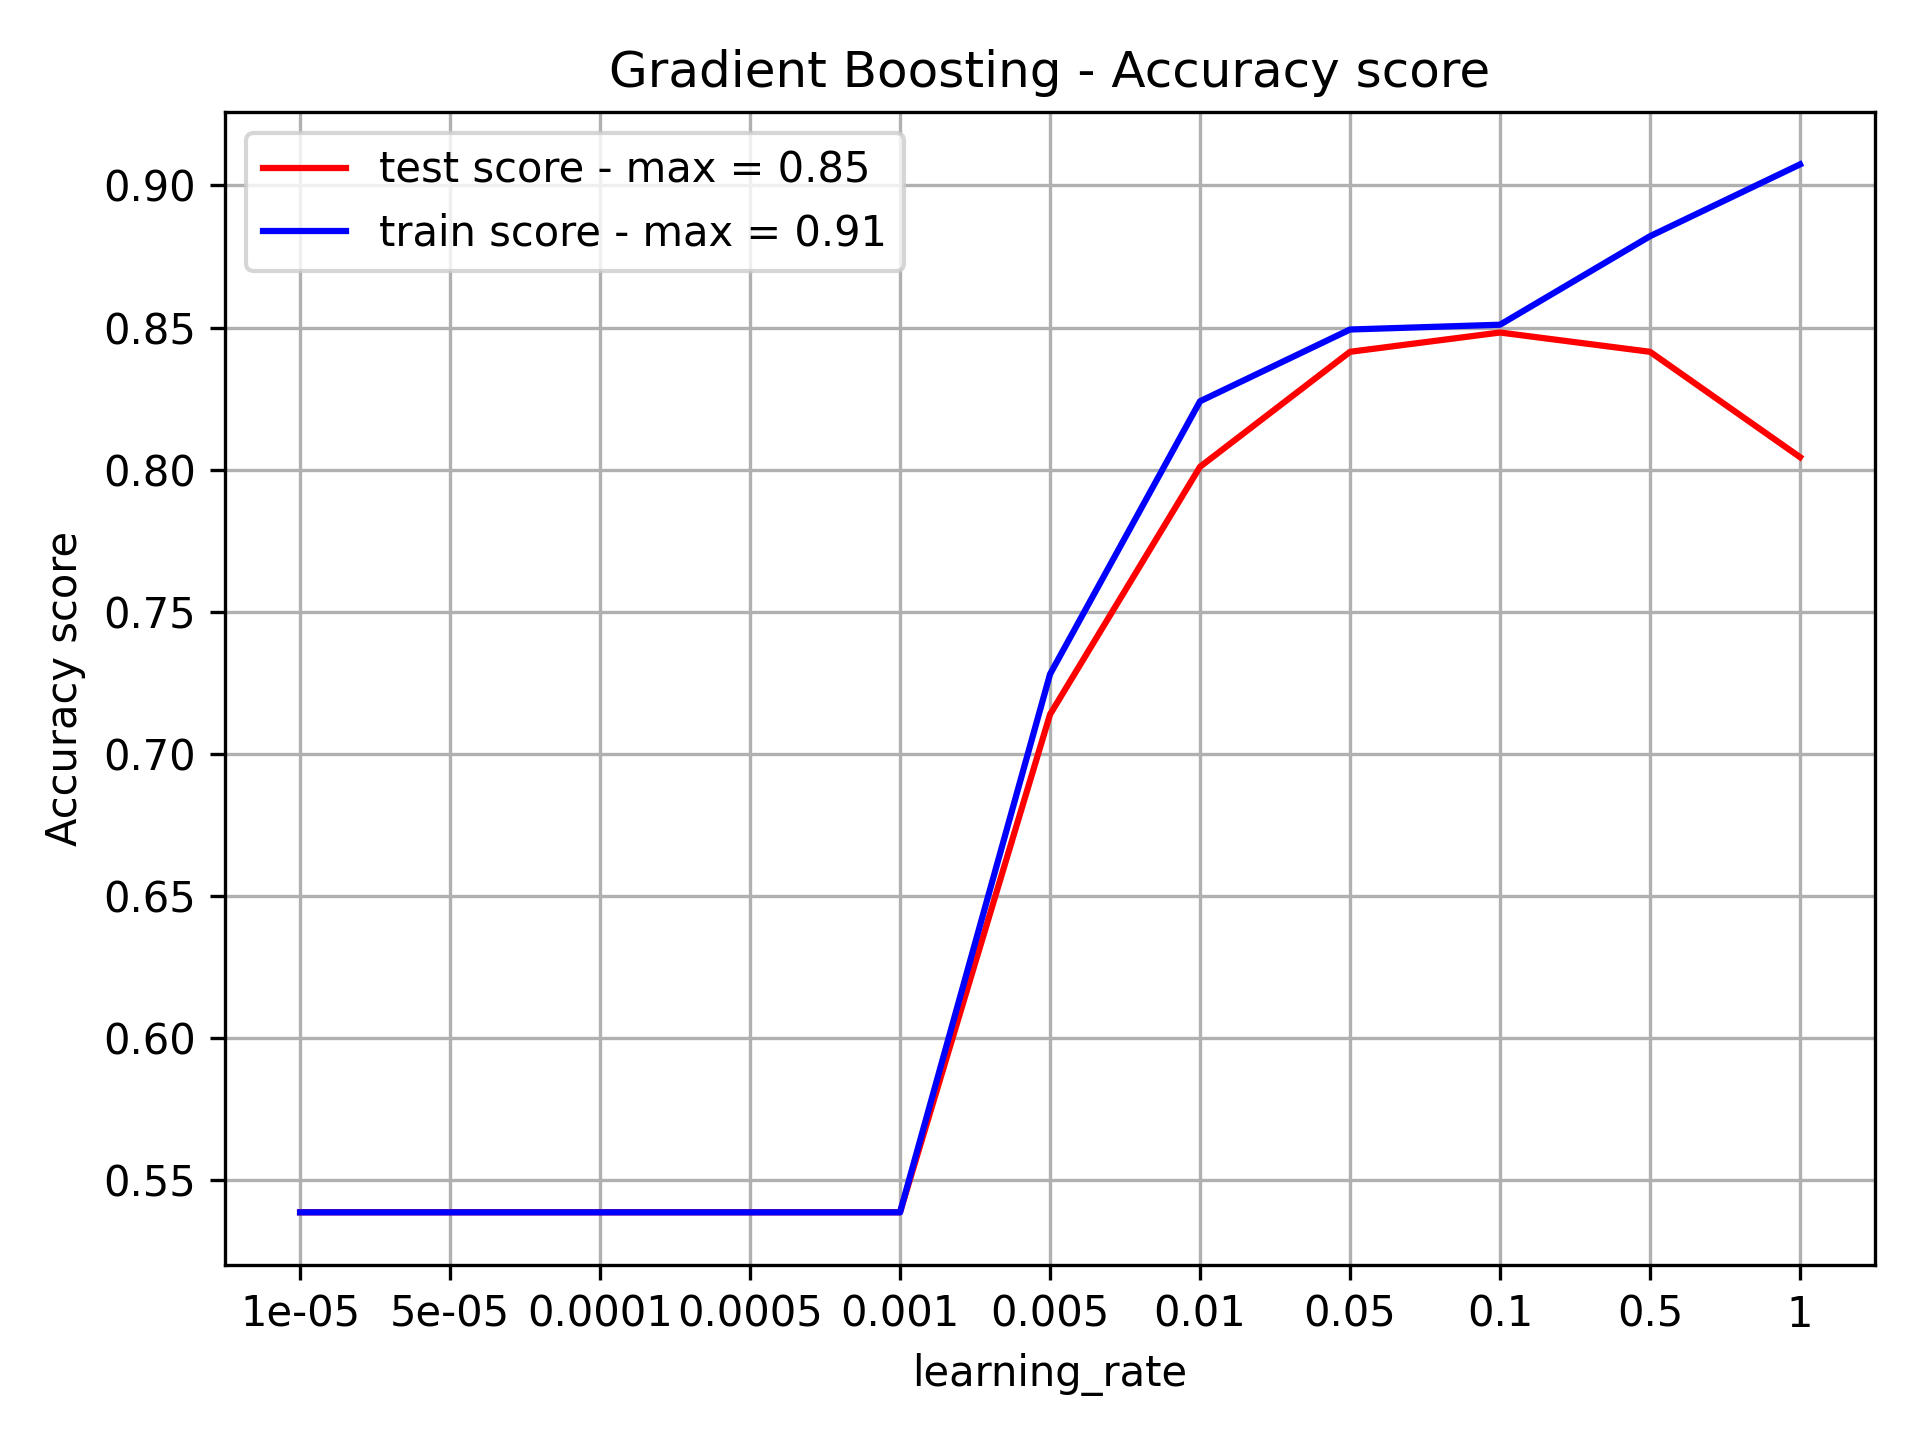
\includegraphics[width=\columnwidth]{gbm_learning_rate_vs_accuracy.png}
    \caption{Figure 13 plots the accuracy score for both the training and test set as a function of $learning\_rate$, with a Gradient Boosting model using the parameters n estimators = 50, max features = log2, max depth = 10 and min samples leaf = 0.3.}
    \label{fig:13}
\end{figure}\\
\\
Similar to AdaBoost, the gradient boosting classifier performs worse for lower learning rates due to not being able to "learn" quickly enough. Both the training accuracy and test accuracy increases as the learning rate increases until a certain point where the learning rate is too large causing the classifier to overfit to the training set. Therefore the training accuracy and test accuracy starts to diverge. A noteworthy difference being that the gradient boosting classifier seems to be more stable for a larger range of learning rates and the test accuracy does not deteriorate as quickly as in figure \ref{fig:11} with AdaBoost.\\
\begin{figure}[!ht]
    \centering
    \begin{subfigure}[b]{\columnwidth}
        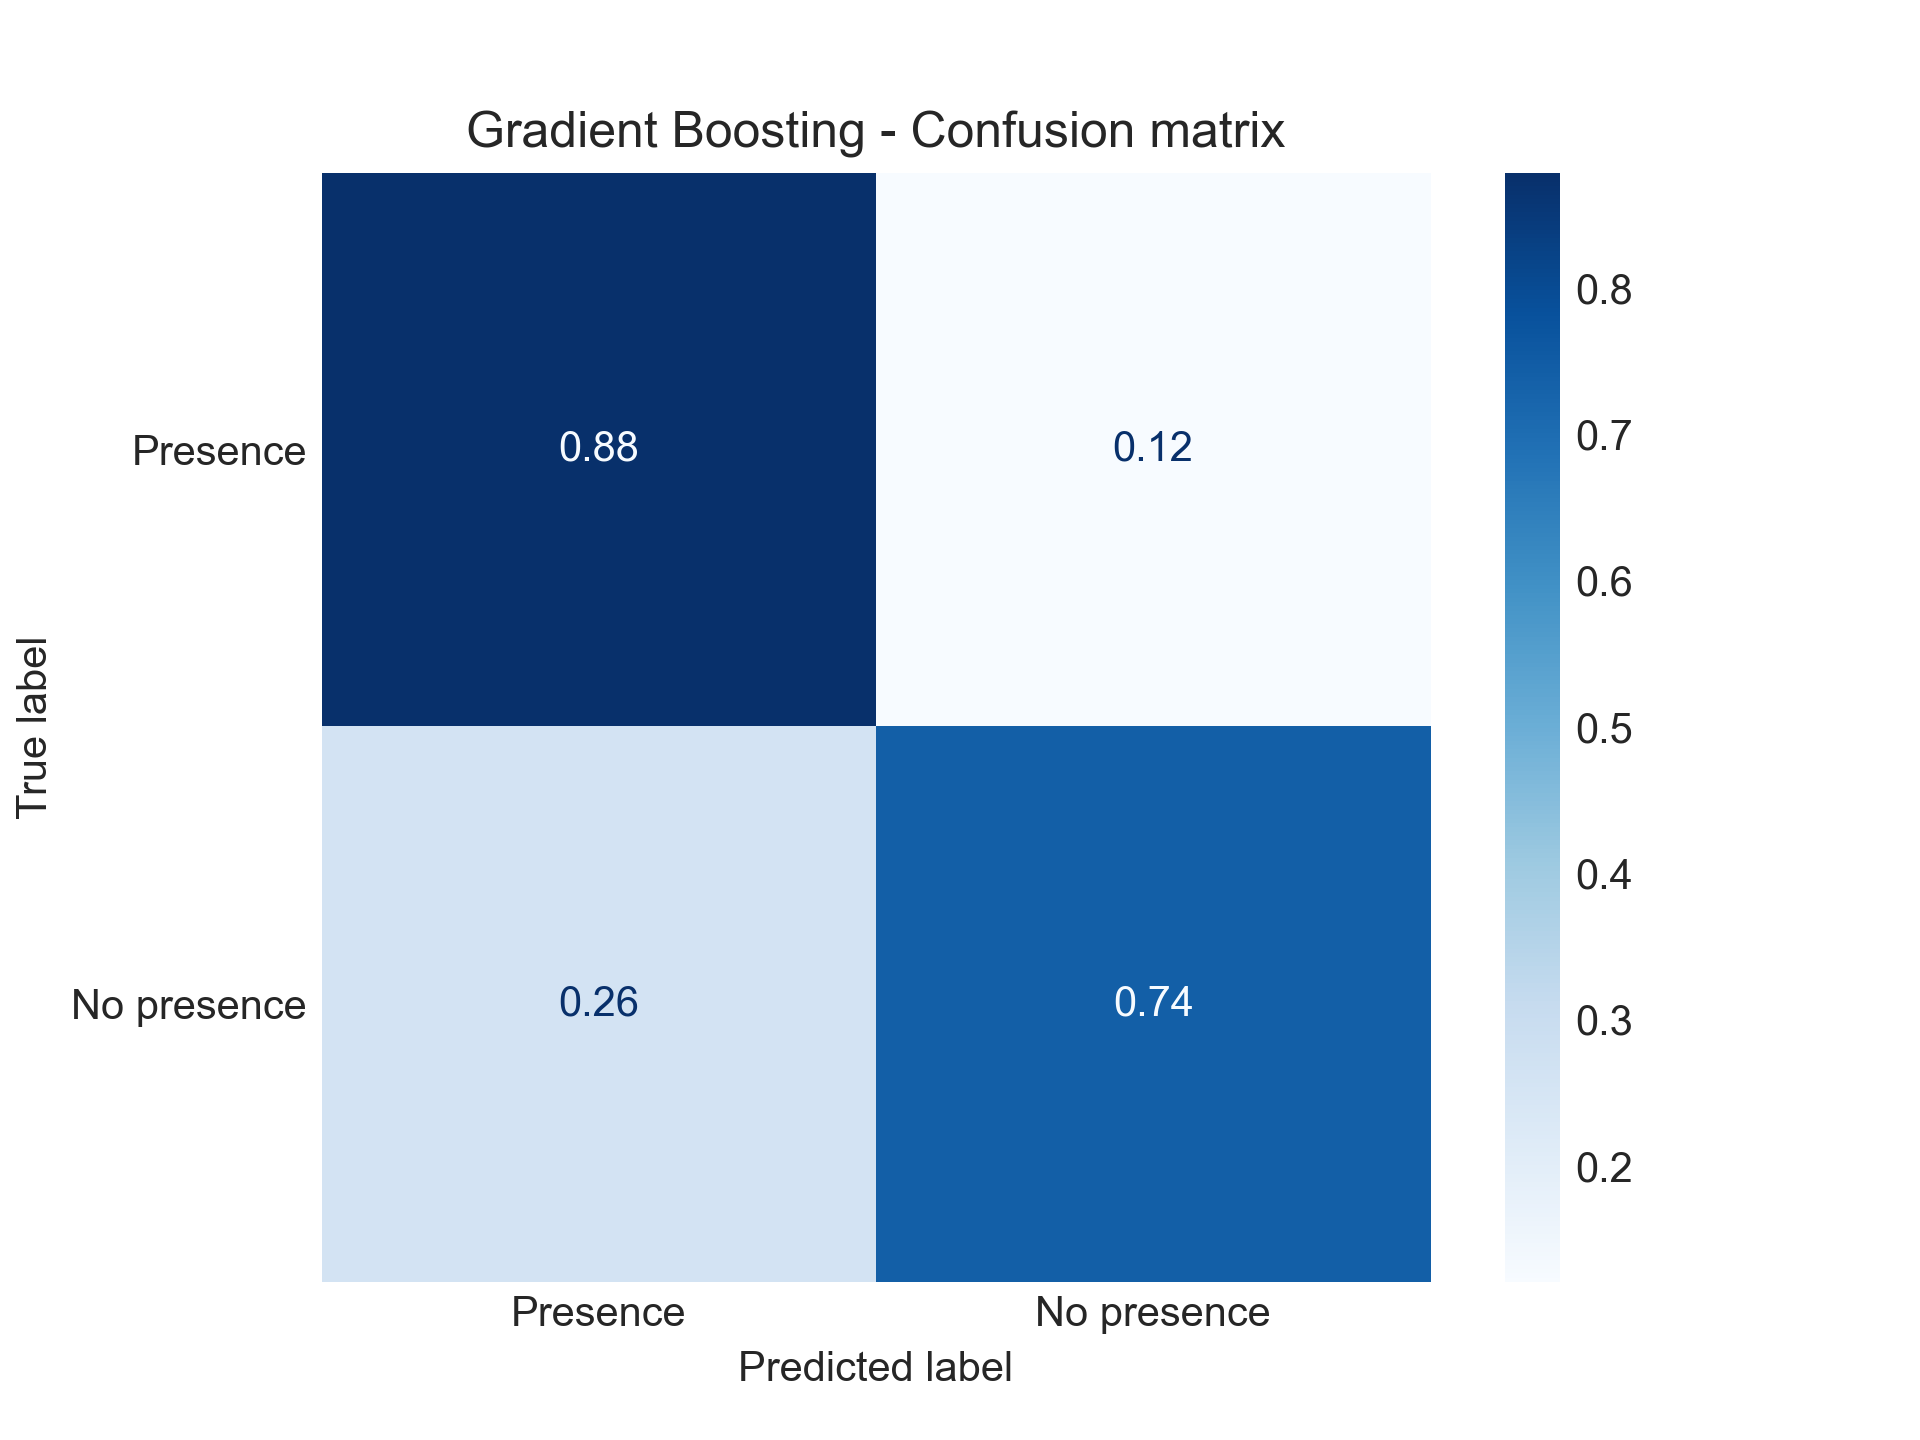
\includegraphics[width=\columnwidth]{gbm_confusion_matrix_learning_rate=0.005_max_depth=5_max_features=log2_min_samples_leaf=0.3_n_estimators=500.png}
        \caption{Confusion matrix with Gradient Boosting using the parameters learning rate=0.005, max depth=5, max features=log2, min samples leaf=0.3 and n estimators=500.}
        \label{fig:14a}
    \end{subfigure}
    
    \begin{subfigure}[b]{\columnwidth}
        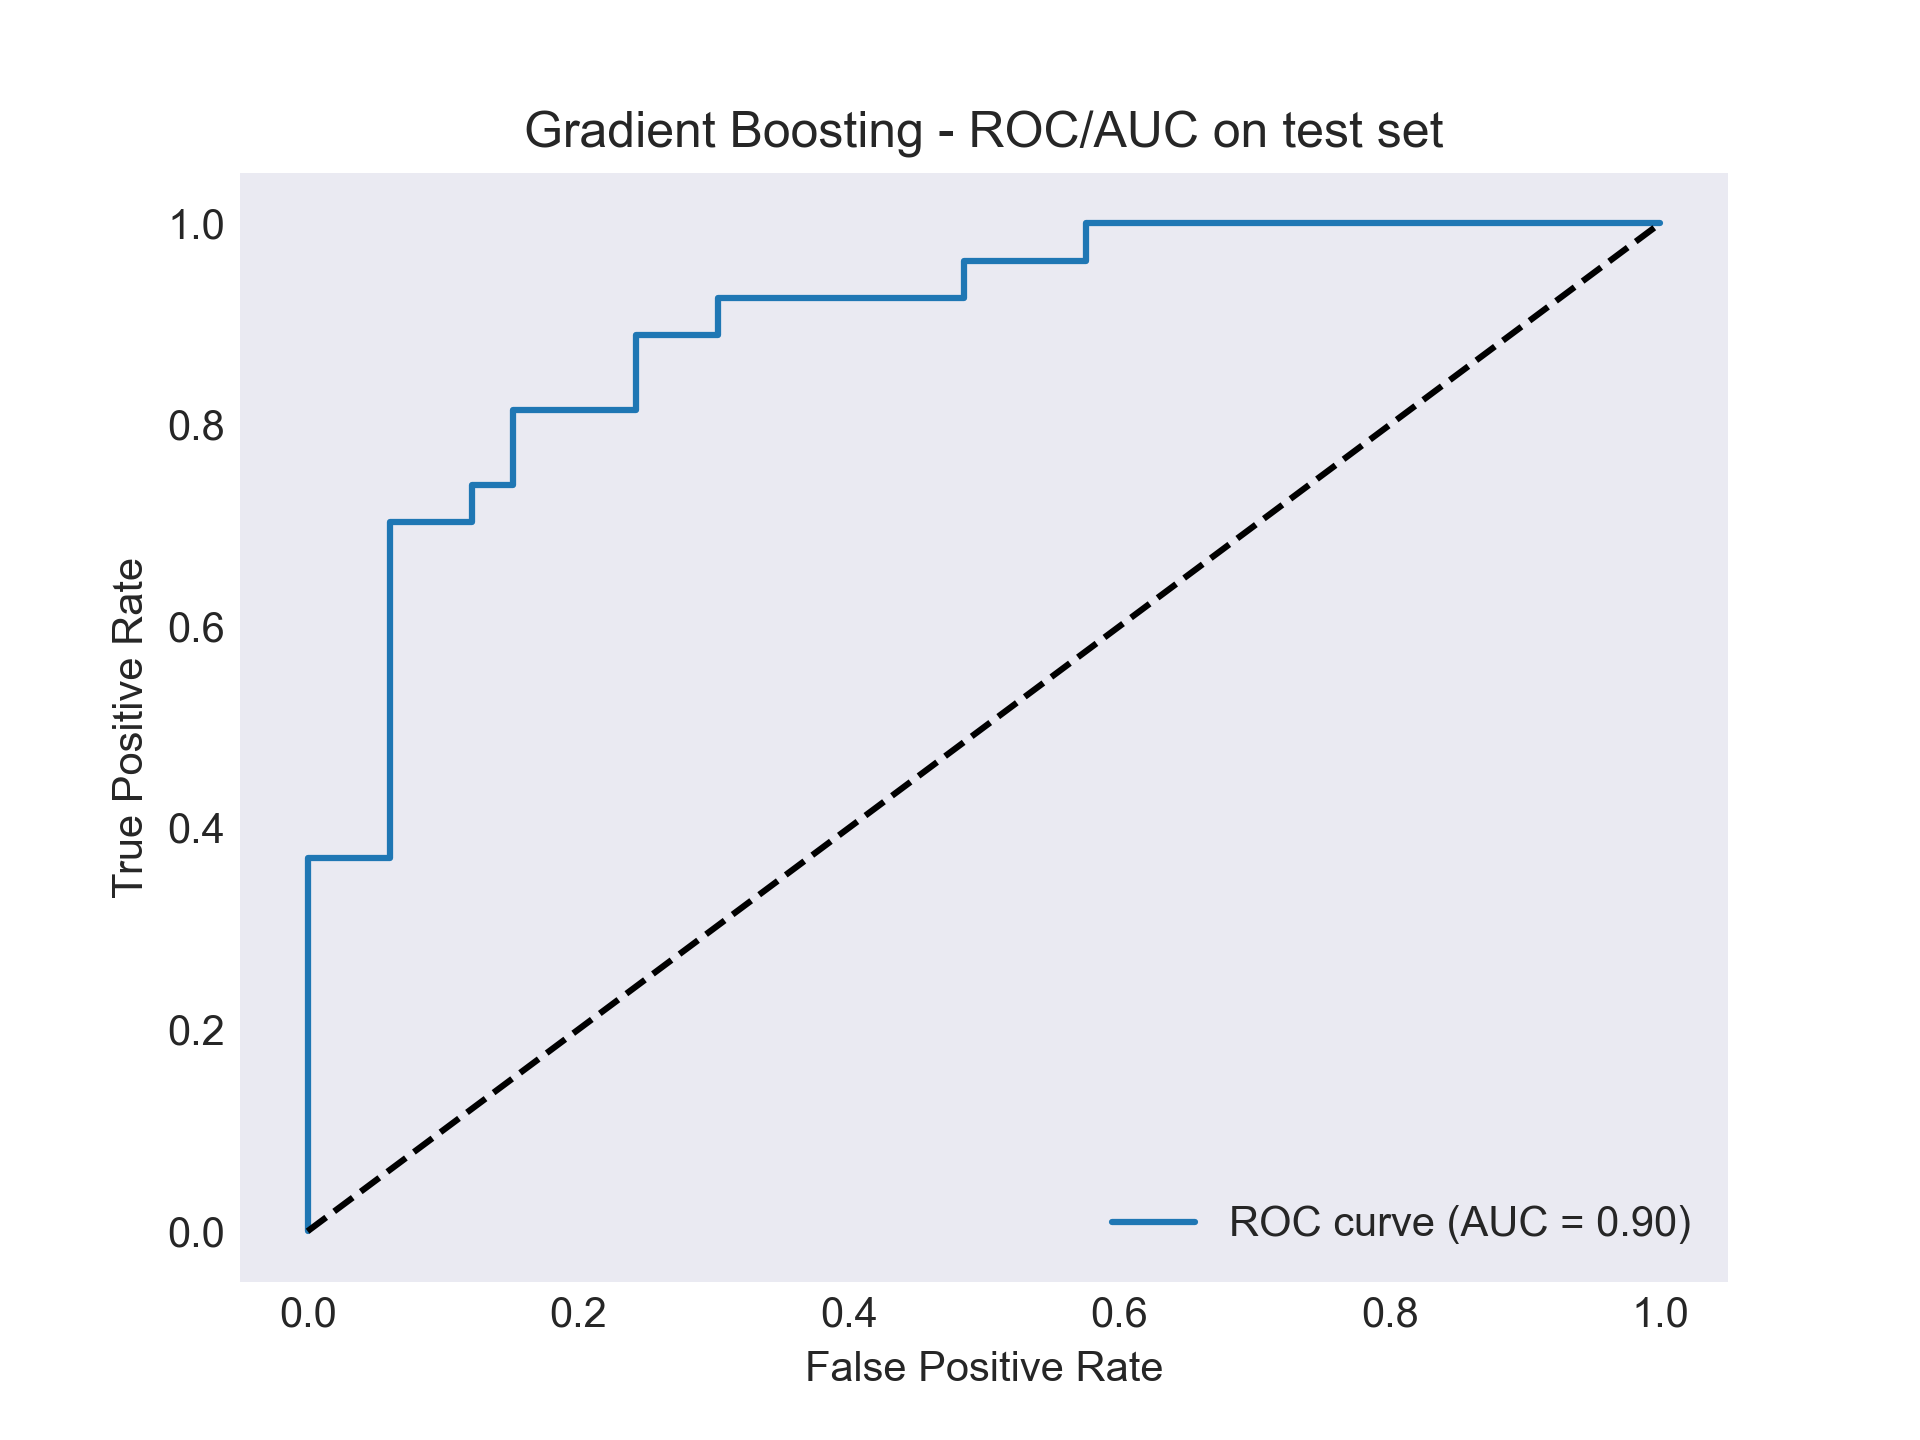
\includegraphics[width=\columnwidth]{gbm_roc_curve_learning_rate=0.005_max_depth=5_max_features=log2_min_samples_leaf=0.3_n_estimators=500.png}
        \caption{ROC curve with Gradient Boosting using the parameters learning rate=0.005, max depth=5, max features=log2, min samples leaf=0.3 and n estimators=500.}
        \label{fig:12b}
    \end{subfigure}
    \caption{14(a) plots the confusion matrix using Gradient Boosting on an untouched test set. 12(b) plots the ROC curve and shows the AUC using Gradient Boosting on an untouched test set. For both figures, the parameters achieving the best test score in table \ref{tab:5} is used.}
    \label{fig:14}
\end{figure}\\
Studying the confusion matrix and ROC curve plotted in figure \ref{fig:14}, we see that gradient boosting achieves a slightly improved classification ratio on instances with heart disease presence but worse on instances with no heart disease presence compared to AdaBoost. While the increased number of correct classification on instances with heart disease presence is beneficial and also the most important, it is wieghed down by the decrease in correct classification on instances ith no heart disease presence. The ROC curve and AUC score for gradient boosting is also similar to AdaBoost and random forests. \\
\\
It should be clarified once again that AdaBoost is a variant of gradient boosting with exponential loss as the loss function. Therefore the similarities between AdaBoost and general gradient boosting is not surprising.\\
\\
The common denominator between random forests and the boosting methods experimented with on the dataset, is that the maximum accuracy achieved seems to be limited to $0.85$ or $0.86$ on the test set. No matter which parameters are used for each classification method, there seems to be an upper bound on the accuracy possible to achieve using the chosen classification methods. There could be multiple explanations for this.\\
\\
One likely explanation is that the classification methods needs more training data. Earlier, an article\cite{introarticle} which explores similar classification methods on heart disease data was presented and the authors were able to achieve an accuracy greater than $0.95$ with both random forests and gradient boosting. The authors of this particular article combined three heart disease datasets, and therefore was able train on more samples. Having more data would help the classifiers adaptability and generalize enough to perform better on an unseen test set.
\\
\\
Also in the aforementioned article, a different machine learning library was used called \textit{Apache Spark}. The implementations in this particular library could perform better than Scikit's implementations.\\
\\
Another explanation, although more unlikely due to the dataset being created by medical experts, could be that the dataset contains outliers that affect the models. This would be counteracted if the dataset was larger. Outliers, especially on smaller datasets, makes it harder for the classification model to more clearly separate the classes.
\newpage
\section{Conclusion}
\subsection{Summary}
The performance of decision trees on the heart disease dataset was found to not be satisfactory. As was shown in the results, decision trees are far too prone to overfitting to be considered an adequate classifier on the heart disease dataset. Random forests, with the ability to reduce the variance and therefore prevent overfitting, achieved significantly better results. The boosting methods used in the project was found to perform on par with random forests, with AdaBoost slightly outperforming random forests and gradient boosting. Overall random forests and boosting methods were less to prone to overfitting and required less tuning of parameters.\\
\\
A maximum accuracy score of $0.86$ on the test set is decent. However we were not able to replicate the results achieved in a recent article\cite{introarticle} using decision trees, random forests and gradient boosting authored by Anna Karen Gárate-Escamila, Amir Hajjam El Hassani and Emmanuel Andrès. Seeing as the classification task concerns heart disease, the accuracy of the classifier is critical. Still, classification methods such as the ones presented in this project are still valuable and useful tools to help doctors and medical experts diagnose more accurately.
\subsection{Future prospects}
Future prospects would be to repeat the experiment but combine multiple dataset to see if the performance improves. Having more data to train the classification models on would likely only increase the accuracy. Also some new methods to try would be extreme gradient boosting, shortened to XGBoost. The library XGBoost has recently impressed many by winning multiple machine learning competitions. It would be interesting to see the performance of XGBoost on the heart disease dataset.
\newpage
\begin{thebibliography}{9}
\bibitem{who}
World Health Organization. (17 May, 2017). Cardiovascular diseases (CVDs). \url{https://www.who.int/news-room/fact-sheets/detail/cardiovascular-diseases-(cvds)}

\bibitem{introarticle}
Gárate-Escamila, A.K. \& El Hassani, A.H. \& Andrès, E. (2020). Classification models for heart disease prediction using feature selection and PCA. Informatics in Medicine Unlocked, Volume 19. \url{https://doi.org/10.1016/j.imu.2020.100330}

\bibitem{scikit}
Scikit-Learn developers. API Reference. \url{https://scikit-learn.org/stable/modules/classes.html}

\bibitem{hastie}
Hastie, T. et al. (2017). The Elements of Statistical Learning, Second Edition. Springer. 

\bibitem{adaboost}
Freund, Y. \& Schapire, R.E. (1997). A Decision-Theoretic Generalization of On-Line Learning and an Application to Boosting. Journal of Computer and System Sciences, Volume 55. \url{https://doi.org/10.1006/jcss.1997.1504}

\bibitem{dataset}
UCI Machine Learning Repository. (1988). Heart Disease Data Set[Dataset, Dataset description]. \url{https://archive.ics.uci.edu/ml/datasets/heart+disease}
\end{thebibliography}
\begin{appendices}
    \section{Derivation of $\mathbf{\alpha_{m}}$ - Adaboost}\label{app:A}
    Our function is defined as 
    \begin{align}
        G(x)=sign\sum_{m=1}^{M}\alpha_{m}G_{m}(x)
    \end{align}
    The iterative procedure is defined as
    \begin{align}
        f_{m}(x) = f_{m-1}(x) + \alpha_{m}G_{m}(x)
    \end{align}
    The choice of cost function in the AdaBoost algorithm is the exponential cost/loss function. The cost function is defined as
    \begin{align}
        C(\mathbf{y}, \mathbf{f}) = \sum_{i=0}^{n-1}exp(-y_{i}(f_{m-1}(x_{i})+\alpha G(x_{i}))
    \end{align}
    The cost function is rewritten as
    \begin{align}
        C(\mathbf{y}, \mathbf{f}) = \sum_{i=0}^{n-1}w_{i}^{m}exp(-y_{i}\alpha G(x_{i}))
    \end{align}
    where we set $w_{i}=exp(-y_{i}f_{m-1}(x_{i}))$. Optimizing $G$ by writing 
    \begin{align}
        G_{m}(x)=sign\sum_{m=1}^{M}w_{i}^{m}I(y_{i} \neq G(x_{i}))
    \end{align}
    where $G_{m}$ is the classifier that minimizes the weighted error. Taking the derivative w.r.t. $\alpha$ we get
    \begin{align}
        \frac{d}{d\alpha} &= exp(-\alpha)\left(\sum_{y_{i}=G({x}_{i})} w_{i}^{m}\right) + exp(\alpha)\left(\sum_{y_{i}\neq G({x}_{i})} w_{i}^{m}\right)
    \end{align}
    Setting the derivative equal to zero
    \begin{align}
        exp(-\alpha)\left(\sum_{y_{i}=G({x}_{i})} w_{i}^{m}\right) + exp(\alpha)\left(\sum_{y_{i}\neq G({x}_{i})} w_{i}^{m}\right) = 0
    \end{align}
    The last step is to solve equation (15) for $\alpha$. Rewrite to
    \begin{align*}
        (exp(\alpha) - exp(-\alpha))&\sum_{i=0}^{n-1}w_{i}^{m}I(y_{i} \neq G(x_{i}))\\
        &+ exp(-\alpha)\sum_{i=0}^{n-1}w_{i}^{m} = 0
    \end{align*}
    which can be solved for $\alpha$ using equation (6) as $\overline{err}_{m}$
    \begin{align}
        \alpha_{m} = \frac{1}{2}log\left(\frac{1- \overline{err}_{m}}{\overline{err}_{m}}\right)
    \end{align}
    \newpage
    \onecolumn
    \section{Feature histograms}\label{app:B}
    \begin{figure}[ht!]
    \centering
    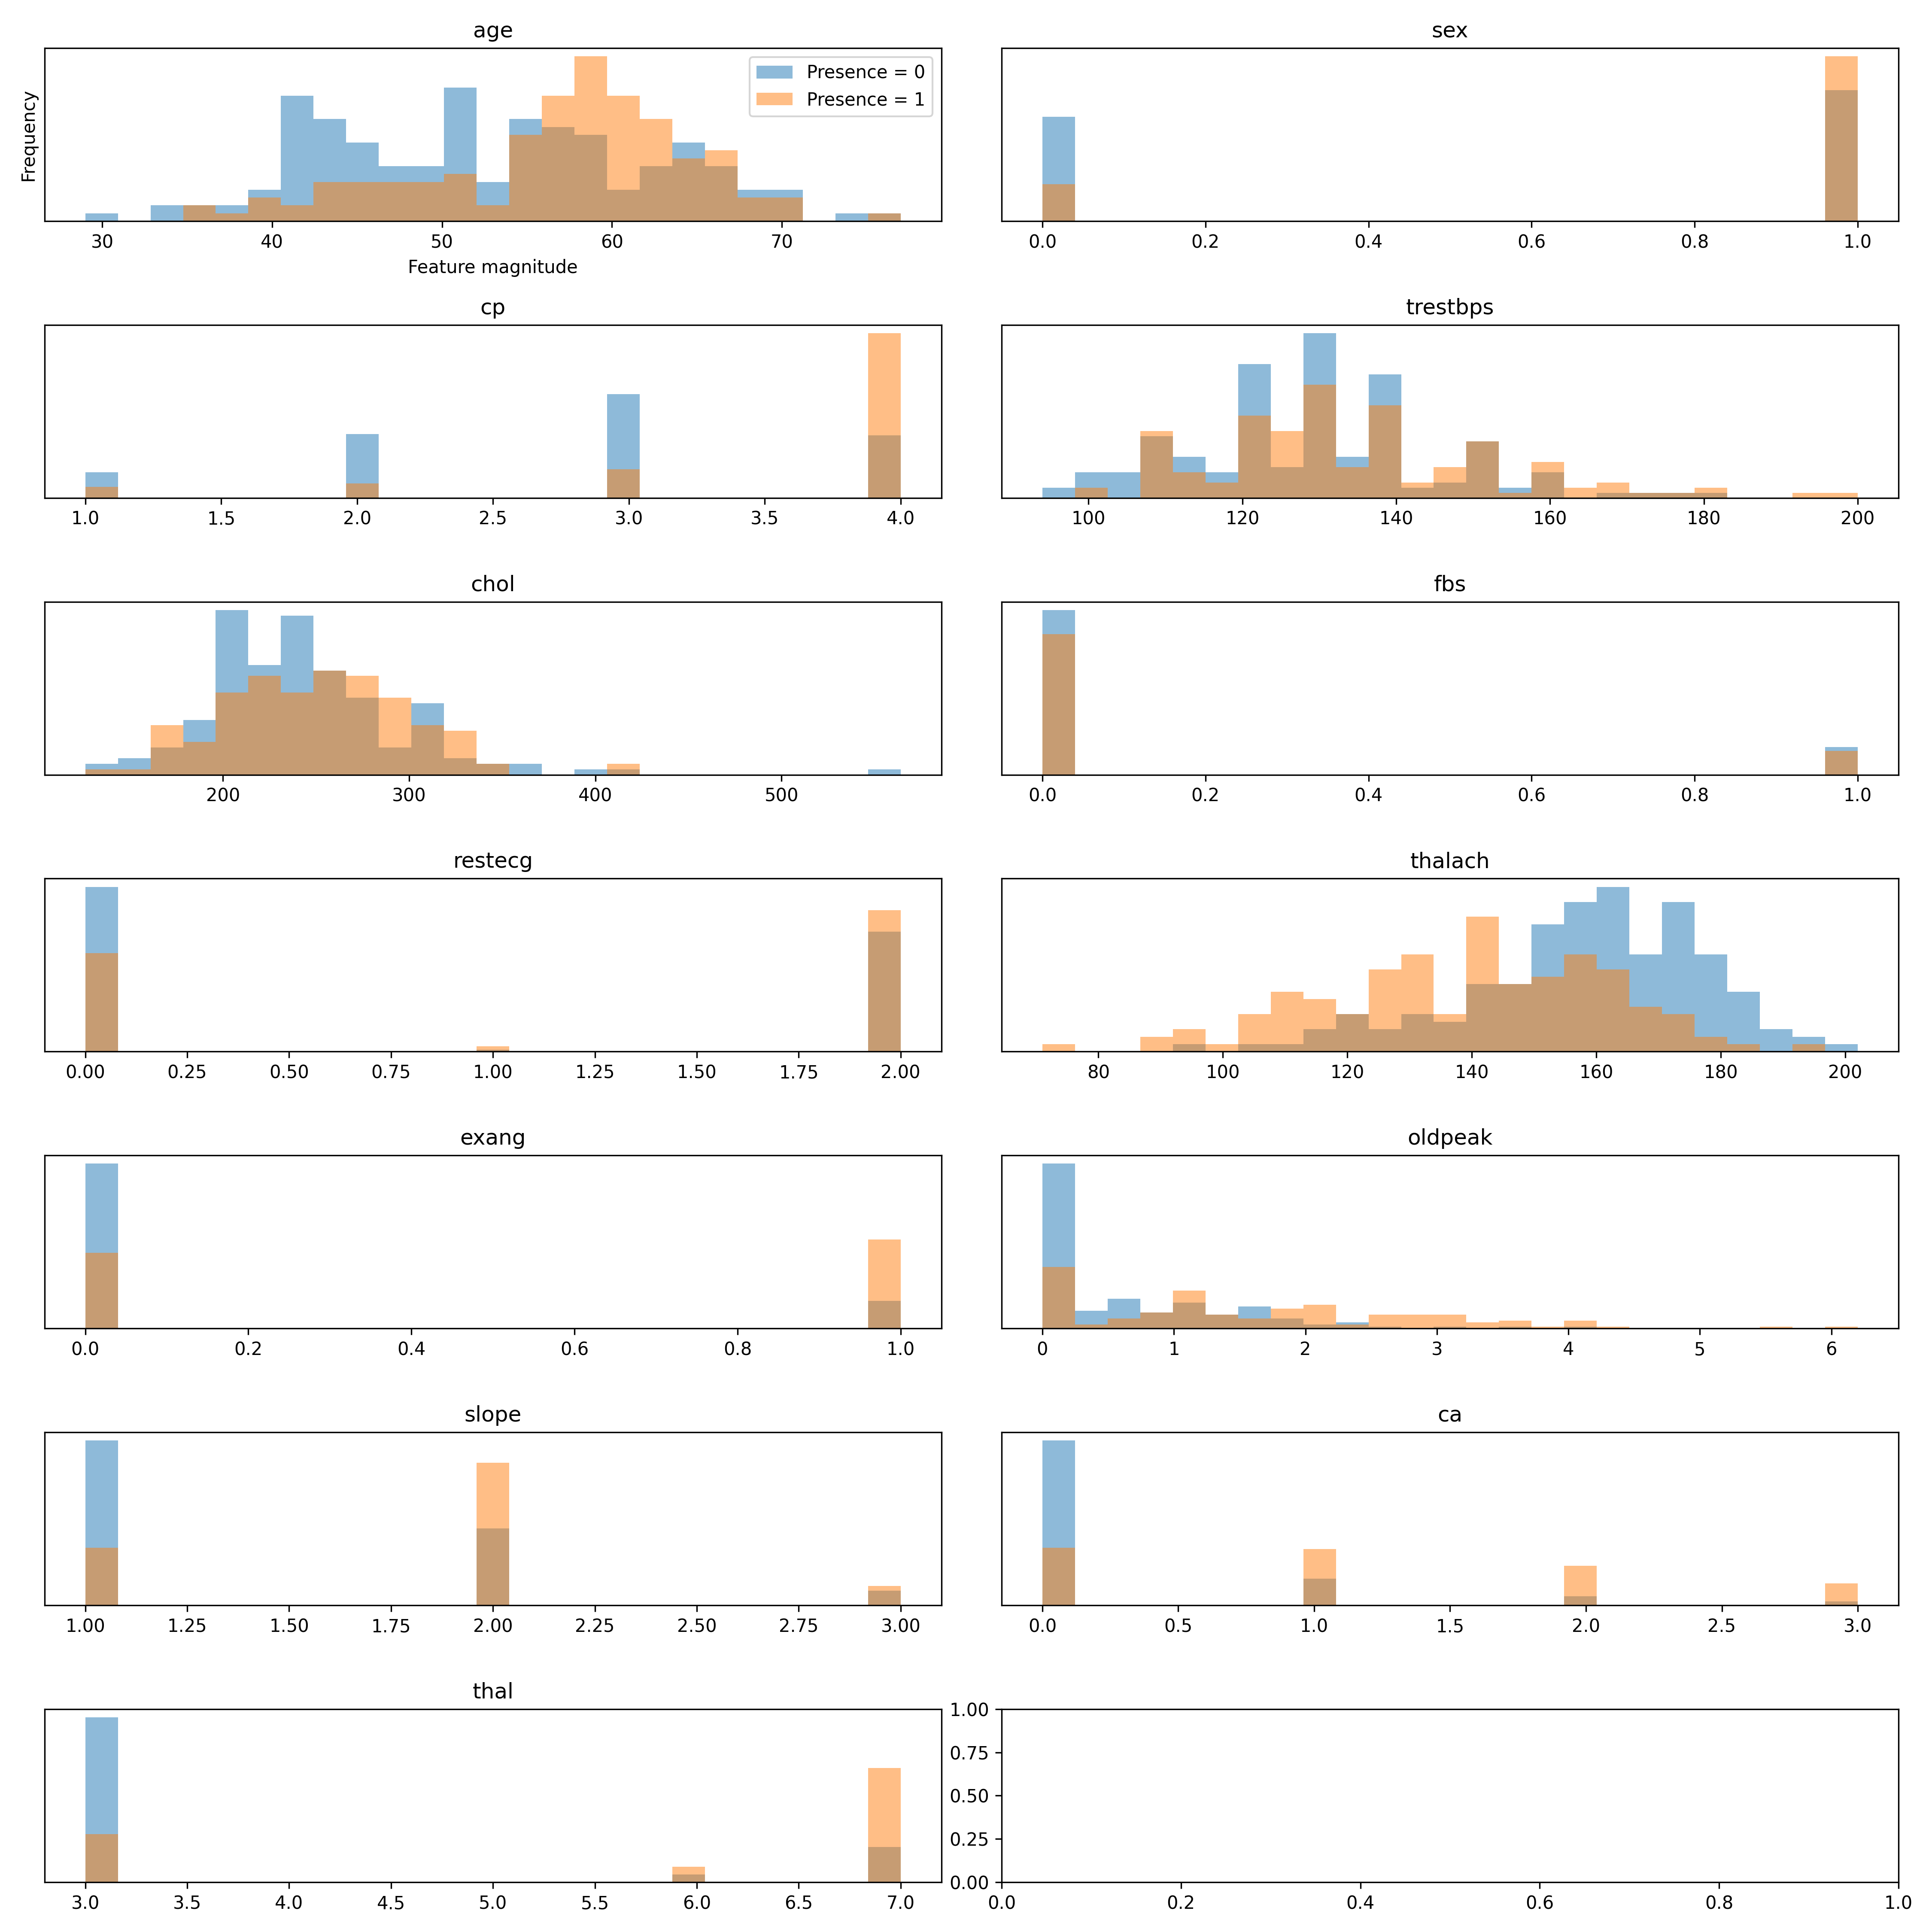
\includegraphics[width=\textwidth]{heart_disease_feature_histograms.png}
    \caption{Histogram for both heart disease presence (light blue) and no heart disease presence (orange) plotted for each feature.}
    \end{figure}
\end{appendices}
\end{document}
